%%%%%%%%%%%%%%%%%%%%%%%%%%%%%%%%%%%%
% Slide options
%%%%%%%%%%%%%%%%%%%%%%%%%%%%%%%%%%%%

% Option 1: Slides with solutions

\documentclass[slidestop,compress,mathserif]{beamer}
\newcommand{\soln}[1]{\textit{#1}}
\newcommand{\solnGr}[1]{#1}

% Option 2: Handouts without solutions

%\documentclass[11pt,containsverbatim,handout]{beamer}
%\usepackage{pgfpages}
%\pgfpagesuselayout{4 on 1}[letterpaper,landscape,border shrink=5mm]
%\newcommand{\soln}[1]{ }
%\newcommand{\solnGr}{ }

%%%%%%%%%%%%%%%%%%%%%%%%%%%%%%%%%%%%
% Style
%%%%%%%%%%%%%%%%%%%%%%%%%%%%%%%%%%%%

\usetheme{metropolis}

%%%%%%%%%%%%%%%%
% Packages
%%%%%%%%%%%%%%%%

\usepackage{geometry}
\usepackage{graphicx}
\usepackage{amssymb}
%\usepackage{cancel}
\usepackage{epstopdf}
\usepackage{amsmath}  	% this permits text in eqnarray among other benefits
\usepackage{url}		% produces hyperlinks
\usepackage{hyperref}	% allows for color usage in tables
\usepackage[english]{babel}
\usepackage[latin1]{inputenc}
\usepackage{colortbl}	% allows for color usage in tables
\usepackage{multirow}	% allows for rows that span multiple rows in tables
\usepackage{color}		% this package has a variety of color options
\usepackage{pgf}
\usepackage{calc}
\usepackage{ulem}
\usepackage{multicol}
\usepackage{textcomp}
\usepackage{txfonts}
\usepackage{listings}
\usepackage{tikz}
\usepackage{array}
\usepackage{wasysym}
\usepackage{fancyvrb}


%%%%%%%%%%%%%%%%
% Remove navigation symbols
%%%%%%%%%%%%%%%%

\setbeamertemplate{navigation symbols}{}

%%%%%%%%%%%%%%%%
% User defined colors
%%%%%%%%%%%%%%%%

\xdefinecolor{oiB}{rgb}{0.22,0.52,0.72}
\definecolor{oiG}{rgb}{.298,.447,.114}
\xdefinecolor{hlblue}{rgb}{0.051,0.65,1}
\xdefinecolor{gray}{rgb}{0.5, 0.5, 0.5}
\xdefinecolor{darkGray}{rgb}{0.3, 0.3, 0.3}
\xdefinecolor{darkerGray}{rgb}{0.2, 0.2, 0.2}
\xdefinecolor{rubineRed}{rgb}{0.89,0,0.30}
\xdefinecolor{irishGreen}{rgb}{0,0.60,0}	
\definecolor{lightGreen}{rgb}{0.387,0.581,0.148} 

%%%%%%%%%%%%%%%%
% Template colors
%%%%%%%%%%%%%%%%

%\setbeamercolor*{palette primary}{fg=white,bg= oiB!80!black!90}
%\setbeamercolor*{palette secondary}{fg=black,bg= oiB!80!black}
%\setbeamercolor*{palette tertiary}{fg=white,bg= oiB!80!black!80}
%\setbeamercolor*{palette quaternary}{fg=white,bg= oiB}
%\setbeamercolor{structure}{fg= oiB}
%\setbeamercolor{frametitle}{bg= oiB!90}
%\setbeamertemplate{blocks}[shadow=false]
%\setbeamersize{text margin left=2em,text margin right=2em}

%\setbeamercolor{code body}{bg=gray!20!white!80,fg=black}


%%%%%%%%%%%%%%%%
% Get rid of fancy enumerated list bullets
%%%%%%%%%%%%%%%%

%\setbeamertemplate{enumerate items}[default]

%%%%%%%%%%%%%%%%
% Custom commands
%%%%%%%%%%%%%%%%

% degree
\newcommand{\degree}{\ensuremath{^\circ}}

% cite
\newcommand{\ct}[1]{
\vfill
{\tiny #1}}

% Note
\newcommand{\Note}[1]{
\rule{2.5cm}{0.25pt} \\ \textit{\footnotesize{\textcolor{rubineRed}{Note:} \textcolor{darkerGray}{#1}}}}

% Remember
\newcommand{\Remember}[1]{\textit{\scriptsize{\textcolor{orange}{Remember:} #1}}}

% expected counts
\newcommand{\ex}[1]{\textit{\textcolor{blue}{#1}}}

% red
\newcommand{\red}[1]{\textit{\textcolor{rubineRed}{#1}}}

% pink
\newcommand{\pink}[1]{\textit{\textcolor{rubineRed!90!white!50}{#1}}}

% green
\newcommand{\green}[1]{\textit{\textcolor{irishGreen}{#1}}}

% orange
\newcommand{\orange}[1]{\textit{\textcolor{orange}{#1}}}

% links: webURL, webLin, appLink
\newcommand{\webURL}[1]{\urlstyle{same}{ \textit{\textcolor{darkGray}{\url{#1}}}}}
\newcommand{\webLink}[2]{\href{#1}{\textcolor{darkGray}{{#2}}}}
\newcommand{\appLink}[2]{\href{#1}{\textcolor{white}{{#2}}}}

% mail
\newcommand{\mail}[1]{\href{mailto:#1}{\textit{\textcolor{darkGray}{#1}}}}

% highlighting: hl, hlGr, mathhl
\newcommand{\hl}[1]{\textit{\textcolor{hlblue}{#1}}}
\newcommand{\hlGr}[1]{\textit{\textcolor{lightGreen}{#1}}}
\newcommand{\mathhl}[1]{\textcolor{hlblue}{\ensuremath{#1}}}

% two col: two columns
\newenvironment{twocol}[4]{
\begin{columns}[c]
\column{#1\textwidth}
#3
\column{#2\textwidth}
#4
\end{columns}
}

% slot (for probability calculations)
\newenvironment{slot}[2]{
\begin{array}{c} 
\underline{#1} \\ 
#2
\end{array}
}

% pr: left and right parentheses
\newcommand{\pr}[1]{
\left( #1 \right)
}

% solnMult: solutions for practice questions

\newcommand{\solnMult}[1]{
\item[] \vspace{-0.59cm}
\only<1>{\item #1}
\soln{\only<2->{\item \orange{#1}}}
}

% cancel
\newcommand{\cancel}[1]{%
    \tikz[baseline=(tocancel.base)]{
        \node[inner sep=0pt,outer sep=0pt] (tocancel) {#1};
        \draw[red, line width=0.5mm] (tocancel.south west) -- (tocancel.north east);
    }%
}

% removepagenumbers
\newcommand{\removepagenumbers}{% 
  \setbeamertemplate{footline}{}
}

%%%%%%%%%%%%%%%%
% Custom boxes
%%%%%%%%%%%%%%%%

% app: application exercise

\setbeamercolor{app body}{fg=oiG}

\newcommand{\app}[1]{
\begin{beamerboxesrounded}[shadow = false, lower = app body]{}
#1
\end{beamerboxesrounded}
}

% dq: discussion question

\setbeamercolor{disc ques body}{fg=oiB}

\newcommand{\dq}[1]{
\begin{beamerboxesrounded}[shadow = false, lower = disc ques body]{}
#1
\end{beamerboxesrounded}
}

% pq: practice question

\setbeamercolor{prac ques body}{fg=oiB}

\newcommand{\pq}[1]{
\begin{beamerboxesrounded}[shadow = false, lower = prac ques body]{}
#1
\end{beamerboxesrounded}
}

% formula

\setbeamercolor{formula body}{fg=oiB!55!black!95}

\newcommand{\formula}[1]{
\begin{beamerboxesrounded}[shadow = false, lower = formula body]{}
#1
\end{beamerboxesrounded}
}


%%%%%%%%%%%%%%%%
% Change margin
%%%%%%%%%%%%%%%%

\newenvironment{changemargin}[2]{%
\begin{list}{}{%
\setlength{\topsep}{0pt}%
\setlength{\leftmargin}{#1}%
\setlength{\rightmargin}{#2}%
\setlength{\listparindent}{\parindent}%
\setlength{\itemindent}{\parindent}%
\setlength{\parsep}{\parskip}%
}%
\item}{\end{list}}

%%%%%%%%%%%%%%%%
% Footnote
%%%%%%%%%%%%%%%%

\long\def\symbolfootnote[#1]#2{\begingroup%
\def\thefootnote{\fnsymbol{footnote}}\footnote[#1]{#2}\endgroup}

%%%%%%%%%%%%%%%%
% Commands from the book
%%%%%%%%%%%%%%%%

\newenvironment{data}[1]{\texttt{#1}}{}
\newenvironment{var}[1]{\texttt{#1}}{}
\newenvironment{resp}[1]{\texttt{#1}}{}

%%%%%%%%%%%%%%%%
% Graphics
%%%%%%%%%%%%%%%%

\DeclareGraphicsRule{.tif}{png}{.png}{`convert #1 `dirname #1`/`basename #1 .tif`.png}


%%%%%%%%%%%%%%%%%%%%%%%%%%%%%%%%%%%%
% Preamble
%%%%%%%%%%%%%%%%%%%%%%%%%%%%%%%%%%%%

\title[Chp 5: Inference for numerical data]{Chapter 5: Inference for numerical data}
\author{OpenIntro Statistics, 3rd Edition}
\institute{$\:$ \\ {\footnotesize Slides developed by Mine \c{C}etinkaya-Rundel of OpenIntro. \\
The slides may be copied, edited, and/or shared via the \webLink{http://creativecommons.org/licenses/by-sa/3.0/us/}{CC BY-SA license.} \\
Some images may be included under fair use guidelines (educational purposes).}}
\date{}


%%%%%%%%%%%%%%%%%%%%%%%%%%%%%%%%%%%%
% Begin document
%%%%%%%%%%%%%%%%%%%%%%%%%%%%%%%%%%%%

\begin{document}


%%%%%%%%%%%%%%%%%%%%%%%%%%%%%%%%%%%%
% Title page
%%%%%%%%%%%%%%%%%%%%%%%%%%%%%%%%%%%%

{
\addtocounter{framenumber}{-1} 
{\removepagenumbers 
\usebackgroundtemplate{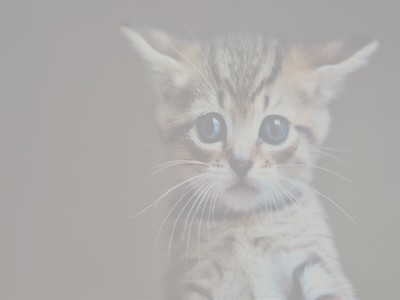
\includegraphics[width=\paperwidth]{../kitten.jpg}}
\begin{frame}

\hfill 
\includegraphics[width=20mm]{../oiLogo_highres}

\titlepage

\end{frame}
}
}


%%%%%%%%%%%%%%%%%%%%%%%%%%%%%%%%%%%%
% Sections
%%%%%%%%%%%%%%%%%%%%%%%%%%%%%%%%%%%%

%%%%%%%%%%%%%%%%%%%%%%%%%%%%%%%%%%%%

\section{One-sample means with the $t$ distribution}

%%%%%%%%%%%%%%%%%%%%%%%%%%%%%%%%%%%%

\begin{frame}
\frametitle{Friday the 13$^{\text{th}}$}

\dq{Between 1990 - 1992 researchers in the UK collected data on traffic flow, accidents, and hospital admissions on Friday 13$^{\text{th}}$ and the previous Friday, Friday 6$^{\text{th}}$. Below is an excerpt from this data set on traffic flow. We can assume that traffic flow on given day at locations 1 and 2 are independent.}

{\scriptsize
\texttt{
\begin{center}
\begin{tabular}{rllrrrl}
  \hline
 & type & date & 6$^{\text{th}}$ & 13$^{\text{th}}$ & diff & location  \\ 
  \hline
1 & traffic & 1990,  July & 139246 & 138548 & 698 & loc 1 \\
  \rowcolor[gray]{.9}
  2 & traffic & 1990,  July & 134012 & 132908 & 1104 & loc 2 \\
  3 & traffic & 1991,  September & 137055 & 136018 & 1037 & loc 1 \\
  \rowcolor[gray]{.9}
  4 & traffic & 1991,  September & 133732 & 131843 & 1889 & loc 2 \\
  5 & traffic & 1991,  December & 123552 & 121641 & 1911 & loc 1 \\
  \rowcolor[gray]{.9}
  6 & traffic & 1991,  December & 121139 & 118723 & 2416 & loc 2 \\
  7 & traffic & 1992,  March & 128293 & 125532 & 2761 & loc 1 \\
  \rowcolor[gray]{.9}
  8 & traffic & 1992,  March & 124631 & 120249 & 4382 & loc 2 \\
  9 & traffic & 1992,  November & 124609 & 122770 & 1839 & loc 1 \\
  \rowcolor[gray]{.9}
  10 & traffic & 1992,  November & 117584 & 117263 & 321 & loc 2 \\
   \hline
\end{tabular}
\end{center}
}}

\vfill

\rule{2.5cm}{0.25pt} \\
{\tiny Scanlon, T.J., Luben, R.N., Scanlon, F.L., Singleton, N. (1993), ``Is Friday the 13th Bad For Your Health?," BMJ, 307, 1584-1586.}

\end{frame}

%%%%%%%%%%%%%%%%%%%%%%%%%%%%%%%%%%%

\begin{frame}
\frametitle{Friday the 13$^{\text{th}}$}

\begin{itemize}

\item We want to investigate if people's behavior is different on Friday 13$^{\text{th}}$ compared to Friday 6$^{\text{th}}$.

\pause

\item One approach is to compare the traffic flow on these two days.

\pause

\item $H_0:$ Average traffic flow on Friday 6$^{\text{th}}$ and 13$^{\text{th}}$ are equal. \\
$H_A:$ Average traffic flow on Friday 6$^{\text{th}}$ and 13$^{\text{th}}$ are different.

\pause

\end{itemize}

$\:$ \\

\dq{Each case in the data set represents traffic flow recorded at the same location in the same month of the same year: one count from Friday 6$^{\text{th}}$ and the other Friday 13$^{\text{th}}$. Are these two counts independent?}

\soln{\pause No}

\end{frame}

%%%%%%%%%%%%%%%%%%%%%%%%%%%%%%%%%%%

\begin{frame}
\frametitle{Hypotheses}

\pq{What are the hypotheses for testing for a difference between the average traffic flow between Friday 6$^{\text{th}}$ and 13$^{\text{th}}$?}

\begin{enumerate}[(a)]
\item  \mathhl{H_0:} $\mu_{6th} = \mu_{13th}$ \\
\mathhl{H_A:} $\mu_{6th} \ne \mu_{13th}$
\item  \mathhl{H_0:} $p_{6th} = p_{13th}$ \\
\mathhl{H_A:} $p_{6th} \ne p_{13th}$
\solnMult{ \mathhl{H_0:} $\mu_{diff} = 0$ \\
\mathhl{H_A:} $\mu_{diff} \ne 0$ }
\item  \mathhl{H_0:} $\bar{x}_{diff} = 0$ \\
\mathhl{H_A:} $\bar{x}_{diff} = 0$
\end{enumerate}

\end{frame}

%%%%%%%%%%%%%%%%%%%%%%%%%%%%%%%%%%%

\begin{frame}
\frametitle{Conditions}

\begin{itemize}

\item \hl{Independence:} We are told to assume that cases (rows) are independent.

\pause

\item \hl{Sample size / skew:} $\:$ \\

\pause

\twocol{0.75}{0.35}
{
{\tiny
\begin{itemize}

\item The sample distribution does not appear to be extremely skewed, but it's very difficult to assess with such a small sample size. We might want to think about whether we would expect the population distribution to be skewed or not -- probably not, it should be equally likely to have days with lower than average traffic and higher than average traffic.

\item We do not know $\sigma$ and $n$ is too small to assume $s$ is a reliable estimate for $\sigma$.
\end{itemize}
}
}
{
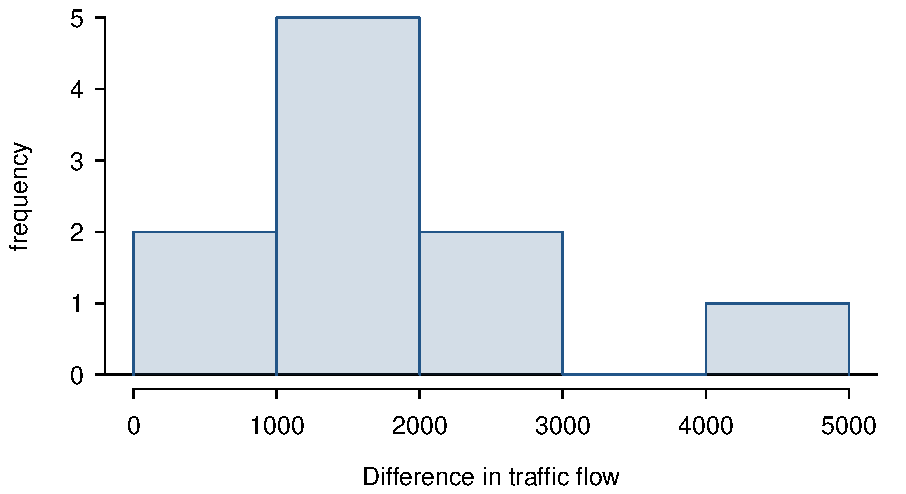
\includegraphics[width=\textwidth]{5-1_one_t/figures/friday/trafficHist}
}

\end{itemize}

$\:$ \\

\pause

\dq{So what do we do when the sample size is small?}

\end{frame}

%%%%%%%%%%%%%%%%%%%%%%%%%%%%%%%%%%%

\begin{frame}
\frametitle{Review: what purpose does a large sample serve?}

As long as observations are independent, and the population distribution is not extremely skewed, a large sample would ensure that...

\begin{itemize}

\item the sampling distribution of the mean is nearly normal

\item the estimate of the standard error, as $\frac{s}{\sqrt{n}}$, is reliable

\end{itemize}

\end{frame}

%%%%%%%%%%%%%%%%%%%%%%%%%%%%%%%%%%%

\subsection{The normality condition}

%%%%%%%%%%%%%%%%%%%%%%%%%%%%%%%%%%%

\begin{frame}
\frametitle{The normality condition}

\begin{itemize}

\item The CLT, which states that sampling distributions will be nearly normal, holds true for \orange{any} sample size as long as the population distribution is nearly normal.

\pause

\item While this is a helpful special case, it's inherently difficult to verify normality in small data sets.

\pause

\item We should exercise caution when verifying the normality condition for small samples. It is important to not only examine the data but also think about where the data come from. 
\begin{itemize}
\item For example, ask: would I expect this distribution to be symmetric, and am I confident that outliers are rare?
\end{itemize}

\end{itemize}

\end{frame}

%%%%%%%%%%%%%%%%%%%%%%%%%%%%%%%%%%%

\subsection{Introducing the $t$ distribution}

%%%%%%%%%%%%%%%%%%%%%%%%%%%%%%%%%%%

\begin{frame}
\frametitle{The $t$ distribution}

\begin{itemize}

\item When the population standard deviation is unknown (almost always), the uncertainty of the standard error estimate is addressed by using a new distribution: the \hl{$t$ distribution}.

\pause

\item This distribution also has a bell shape, but its tails are \hl{thicker} than the normal model's.

\pause

\item Therefore observations are more likely to fall beyond two SDs from the mean than under the normal distribution.

\pause

\item These extra thick tails are helpful for resolving our problem with a less reliable estimate the standard error (since $n$ is small)

\end{itemize}

\begin{center}
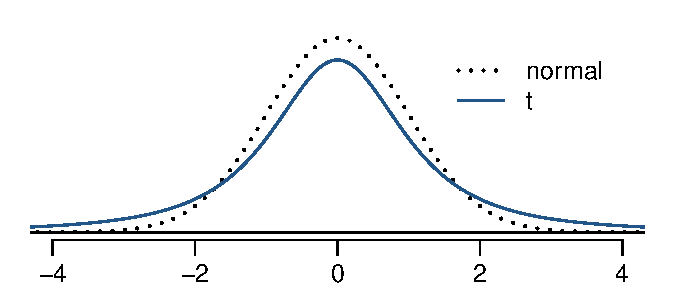
\includegraphics[width=0.5\textwidth]{5-1_one_t/figures/tDistCompareToNormalDist/tDistCompareToNormalDist}
\end{center}

\end{frame}

%%%%%%%%%%%%%%%%%%%%%%%%%%%%%%%%%%%

\begin{frame}
\frametitle{The $t$ distribution (cont.)}

\begin{itemize}

\item Always centered at zero, like the standard normal ($z$) distribution.

\item Has a single parameter: \hl{degrees of freedom} (\mathhl{df}).

\end{itemize}

\begin{center}
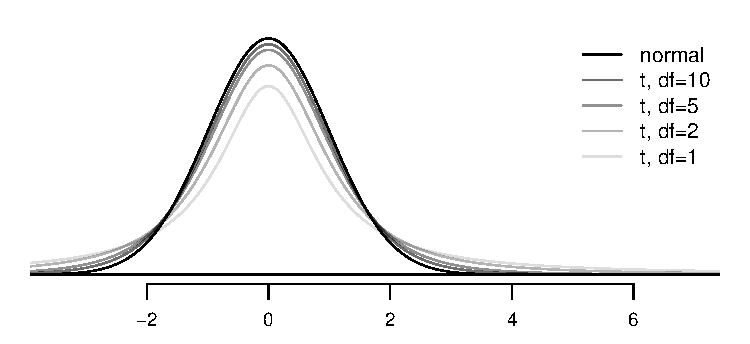
\includegraphics[width=0.8\textwidth]{5-1_one_t/figures/tDistConvergeToNormalDist/tDistConvergeToNormalDist}
\end{center}

\pause

\dq{What happens to shape of the $t$ distribution as $df$ increases?}

\soln{\pause Approaches normal.}

\end{frame}

%%%%%%%%%%%%%%%%%%%%%%%%%%%%%%%%%%%

\subsection{Evaluating hypotheses using the $t$ distribution}

%%%%%%%%%%%%%%%%%%%%%%%%%%%%%%%%%%%

\begin{frame}
\frametitle{Back to Friday the 13$^{\text{th}}$}

{\footnotesize
\texttt{
\begin{center}
\begin{tabular}{rllrr || r || l}
  \hline
 & type & date & 6$^{\text{th}}$ & 13$^{\text{th}}$ & diff & location  \\ 
  \hline
1 & traffic & 1990,  July & 139246 & 138548 & 698 & loc 1 \\
  \rowcolor[gray]{.9}
  2 & traffic & 1990,  July & 134012 & 132908 & 1104 & loc 2 \\
  3 & traffic & 1991,  September & 137055 & 136018 & 1037 & loc 1 \\
  \rowcolor[gray]{.9}
  4 & traffic & 1991,  September & 133732 & 131843 & 1889 & loc 2 \\
  5 & traffic & 1991,  December & 123552 & 121641 & 1911 & loc 1 \\
  \rowcolor[gray]{.9}
  6 & traffic & 1991,  December & 121139 & 118723 & 2416 & loc 2 \\
  7 & traffic & 1992,  March & 128293 & 125532 & 2761 & loc 1 \\
  \rowcolor[gray]{.9}
  8 & traffic & 1992,  March & 124631 & 120249 & 4382 & loc 2 \\
  9 & traffic & 1992,  November & 124609 & 122770 & 1839 & loc 1 \\
  \rowcolor[gray]{.9}
  10 & traffic & 1992,  November & 117584 & 117263 & 321 & loc 2 \\
   \hline
\end{tabular}
\end{center}
}}

\hspace{8.5cm} \orange{$\downarrow$}
\begin{align*}
\hspace{6cm} &\orange{$\bar{x}_{diff} = 1836$} \\
& \orange{$s_{diff} = 1176$} \\
& \orange{$n = 10$} 
\end{align*}
 
\end{frame}

%%%%%%%%%%%%%%%%%%%%%%%%%%%%%%%%%%%

\begin{frame}
\frametitle{Finding the test statistic}

\formula{Test statistic for inference on a small sample mean}
{The test statistic for inference on a small sample ($n < 50$) mean is the $T$ statistic with $df = n - 1$.
\[ T_{df} = \frac{\text{point estimate} - \text{null value}}{SE} \]}

\pause

\vspace{-0.5cm}

\hl{in context...}
\begin{eqnarray*}
point~estimate &=& \bar{x}_{diff} = 1836 \\
\pause
SE &=& \frac{s_{diff}}{\sqrt{n}} = \frac{1176}{\sqrt{10}} = 372 \\
\pause
T &=& \frac{1836 - 0}{372} = 4.94 \\
\pause
df &=& 10 - 1 = 9
\end{eqnarray*}

\Note{Null value is 0 because in the null hypothesis we set $\mu_{diff} = 0$.}

\end{frame}

%%%%%%%%%%%%%%%%%%%%%%%%%%%%%%%%%%%

\begin{frame}[fragile]
\frametitle{Finding the p-value}

\begin{itemize}

\item The p-value is, once again, calculated as the area tail area under the $t$ distribution.

\pause

\item Using R:
\begin{verbatim}
> 2 * pt(4.94, df = 9, lower.tail = FALSE)

[1] 0.0008022394
\end{verbatim}

\pause

\item Using a web app:

\href{https://gallery.shinyapps.io/dist_calc/}{\textcolor{oiB}{https://gallery.shinyapps.io/dist\_calc/}}

\pause

\item Or when these aren't available, we can use a \webLink{https://www.openintro.org/download.php?file=os2_prob_tables&referrer=/stat/textbook.php}{$t$-table}.

\end{itemize}

\end{frame}

%%%%%%%%%%%%%%%%%%%%%%%%%%%%%%%%%%%

\begin{frame}
\frametitle{Finding the p-value}

Locate the calculated $T$ statistic on the appropriate $df$ row, obtain the p-value from the corresponding column heading (one or two tail, depending on the alternative hypothesis).

{\scriptsize
\begin{center}
\begin{tabular}{r | rrr rr}
one tail & \hspace{1.5mm}  0.100 & \hspace{1.5mm} 0.050 & \hspace{1.5mm} 0.025 & \hspace{1.5mm} 0.010 & \hspace{1.5mm} 0.005  \\
two tails & 0.200 & 0.100 & 0.050 & 0.020 & 0.010 \\
\hline
{$df$} \hfill 1  &  {  3.08} & {  6.31} & { 12.71} & { 31.82} & { 63.66}  \\ 
2  &  {  1.89} & {  2.92} & {  4.30} & {  6.96} & {  9.92}  \\ 
3  &  {  1.64} & {  2.35} & {  3.18} & {  4.54} & {  5.84}  \\ 
$\vdots$ & $\vdots$ &$\vdots$ &$\vdots$ &$\vdots$ & \\
17  &  {  1.33} & {  1.74} & {  2.11} & {  2.57} & {  2.90}  \\ 
18  &  {  1.33} & {  1.73} & {  2.10} & {  2.55} & {  2.88}  \\ 
19  &  {  1.33} & {  1.73} & {  2.09} & {  2.54} & {  2.86}  \\ 
20  &  {  1.33} & {  1.72} & {  2.09} & {  2.53} & {  2.85}  \\ 
$\vdots$ & $\vdots$ &$\vdots$ &$\vdots$ &$\vdots$ & \\
400  &  {  1.28} & {  1.65} & {  1.97} & {  2.34} & {  2.59}  \\ 
500  &  {  1.28} & {  1.65} & {  1.96} & {  2.33} & {  2.59}  \\ 
$\infty$  &  {  1.28} & {  1.64} & {  1.96} & {  2.33} & {  2.58}  \\ 
\end{tabular}
\end{center}
}

\end{frame}

%%%%%%%%%%%%%%%%%%%%%%%%%%%%%%%%%%%

\begin{frame}
\frametitle{Finding the p-value (cont.)}

\only<1>{
{\footnotesize
\begin{center}
\begin{tabular}{r | rrr rr}
\hline
one tail & \hspace{1.5mm}  0.100 & \hspace{1.5mm} 0.050 & \hspace{1.5mm} 0.025 & \hspace{1.5mm} 0.010 & \hspace{1.5mm} 0.005  \\
two tails & 0.200 & 0.100 & 0.050 & 0.020 & 0.010 \\
\hline
{df} \hfill 6  &  {  1.44} & {  1.94} & {  2.45} & {  3.14} & {  3.71}  \\ 
7  &  {  1.41} & {  1.89} & {  2.36} & {  3.00} & {  3.50}  \\ 
8  &  {  1.40} & {  1.86} & {  2.31} & {  2.90} & {  3.36}  \\ 
9  &  {  1.38} & {  1.83} & {  2.26} & {  2.82} & {  3.25}  \\ 
10  &  {  1.37} & {  1.81} & {  2.23} & {  2.76} & {  3.17}  \\ 
\end{tabular}
\end{center}
}
}

\only<2 | handout:0>{
{\footnotesize
\begin{center}
\begin{tabular}{r | rrr rr}
\hline
one tail & \hspace{1.5mm}  0.100 & \hspace{1.5mm} 0.050 & \hspace{1.5mm} 0.025 & \hspace{1.5mm} 0.010 & \hspace{1.5mm} 0.005  \\
two tails & 0.200 & 0.100 & 0.050 & 0.020 & 0.010 \\
\hline
{df} \hfill 6  &  {  1.44} & {  1.94} & {  2.45} & {  3.14} & {  3.71}  \\ 
7  &  {  1.41} & {  1.89} & {  2.36} & {  3.00} & {  3.50}  \\ 
8  &  {  1.40} & {  1.86} & {  2.31} & {  2.90} & {  3.36}  \\ 
  \rowcolor[gray]{.6}
9  &  {  1.38} & {  1.83} & {  2.26} & {  2.82} & {  3.25}  \\ 
10  &  {  1.37} & {  1.81} & {  2.23} & {  2.76} & {  3.17}  \\ 
\end{tabular}
\end{center}
}
}

\only<3-| handout:0>{
{\footnotesize
\begin{center}
\begin{tabular}{r | rrr rr r}
\hline
one tail & \hspace{1.5mm}  0.100 & \hspace{1.5mm} 0.050 & \hspace{1.5mm} 0.025 & \hspace{1.5mm} 0.010 & \hspace{1.5mm} 0.005  \\
  \rowcolor[gray]{.6}
two tails & 0.200 & 0.100 & 0.050 & 0.020 & \orange{0.010} & \mathhl{\rightarrow} \\
\hline
{df} \hfill 6  &  {  1.44} & {  1.94} & {  2.45} & {  3.14} & {  3.71}  \\ 
7  &  {  1.41} & {  1.89} & {  2.36} & {  3.00} & {  3.50}  \\ 
8  &  {  1.40} & {  1.86} & {  2.31} & {  2.90} & {  3.36}  \\ 
  \rowcolor[gray]{.6}
9  &  {  1.38} & {  1.83} & {  2.26} & {  2.82} & \orange{  3.25} & \mathhl{\rightarrow}  \\ 
10  &  {  1.37} & {  1.81} & {  2.23} & {  2.76} & {  3.17}  \\ 
\end{tabular}
\end{center}
}
}

\twocol{0.5}{0.5}{
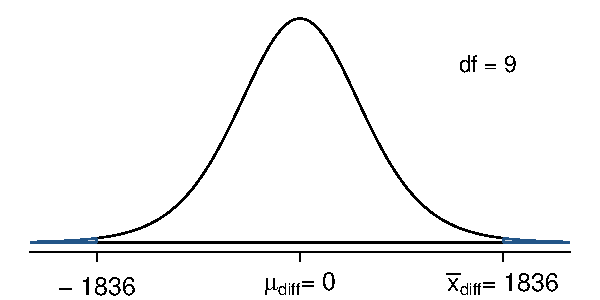
\includegraphics[width=1.1\textwidth]{5-1_one_t/figures/friday/fridayPvalue}
}
{
$T = 4.94$
\only<4->{\dq{What is the conclusion of the hypothesis test?}}
\soln{\only<5>{The data provide convincing evidence of a difference between traffic flow on Friday 6$^{\text{th}}$ and 13$^{\text{th}}$.}}
}

\end{frame}

%%%%%%%%%%%%%%%%%%%%%%%%%%%%%%%%%%%%

\subsection{Constructing confidence intervals using the $t$ distribution}

%%%%%%%%%%%%%%%%%%%%%%%%%%%%%%%%%%%

\begin{frame}
\frametitle{What is the difference?}

\begin{itemize}

\item We concluded that there is a difference in the traffic flow between Friday 6$^{\text{th}}$ and 13$^{\text{th}}$.

\pause

\item But it would be more interesting to find out what exactly this difference is.

\pause

\item We can use a confidence interval to estimate this difference.

\end{itemize}

\end{frame}

%%%%%%%%%%%%%%%%%%%%%%%%%%%%%%%%%%%

\begin{frame}
\frametitle{Confidence interval for a small sample mean}

\begin{itemize}

\item Confidence intervals are always of the form
\[ \text{point estimate} \pm {ME} \]

\pause

\item ME is always calculated as the product of a critical value and SE.

\pause

\item Since small sample means follow a $t$ distribution (and not a $z$ distribution), the critical value is a $t^\star$ (as opposed to a $z^\star$).
\[ \text{point estimate} \pm t^{\star} \times SE \]

\end{itemize}

\end{frame}

%%%%%%%%%%%%%%%%%%%%%%%%%%%%%%%%%%%

\begin{frame}
\frametitle{Finding the critical $t$ ($t^\star$)}

\twocol{0.5}{0.5}{
\only<1-3>{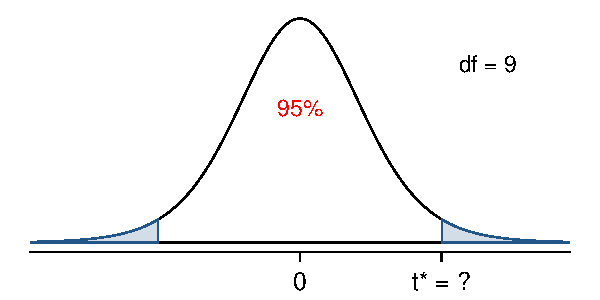
\includegraphics[width=\textwidth]{5-1_one_t/figures/middle95/middle95_1}}
\only<4| handout:0>{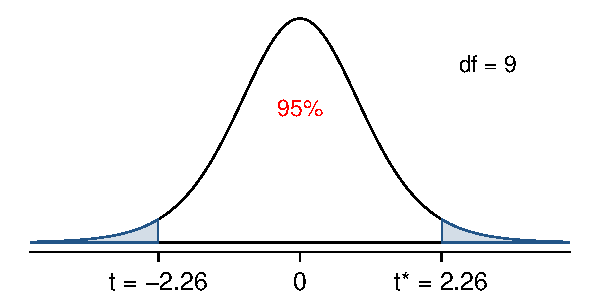
\includegraphics[width=\textwidth]{5-1_one_t/figures/middle95/middle95_2}}
}
{
$n = 10$, $df = 10 - 1 = 9$, $t^\star$ is at the intersection of row $df = 9$ and two tail probability 0.05.
}

\only<1>{
{\small
\begin{center}
\begin{tabular}{r | r r r r r}
\hline
one tail & \hspace{1.5mm}  0.100 & \hspace{1.5mm} 0.050 & \hspace{1.5mm} 0.025 & \hspace{1.5mm} 0.010 & \hspace{1.5mm} 0.005  \\
two tails & 0.200 & 0.100 & 0.050 & 0.020 & {0.010} \\
\hline
{df} \hfill 6  &  {  1.44} & {  1.94} & {  2.45} & {  3.14} & {  3.71}  \\ 
7  &  {  1.41} & {  1.89} & {  2.36} & {  3.00} & {  3.50}  \\ 
8  &  {  1.40} & {  1.86} & {  2.31} & {  2.90} & {  3.36}  \\ 
9  &  {  1.38} & {  1.83} & {  2.26} & {  2.82} & {  3.25} \\ 
10  &  {  1.37} & {  1.81} & {  2.23} & {  2.76} & {  3.17}  \\ 
\end{tabular}
\end{center}
}}

\only<2 | handout:0>{
{\small
\begin{center}
\begin{tabular}{r | r r r r r}
\hline
one tail & \hspace{1.5mm}  0.100 & \hspace{1.5mm} 0.050 & \hspace{1.5mm} 0.025 & \hspace{1.5mm} 0.010 & \hspace{1.5mm} 0.005  \\
two tails & 0.200 & 0.100 & 0.050 & 0.020 & {0.010} \\
\hline
{df} \hfill 6  &  {  1.44} & {  1.94} & {  2.45} & {  3.14} & {  3.71}  \\ 
7  &  {  1.41} & {  1.89} & {  2.36} & {  3.00} & {  3.50}  \\ 
8  &  {  1.40} & {  1.86} & {  2.31} & {  2.90} & {  3.36}  \\ 
  \rowcolor[gray]{.6}
9  &  {  1.38} & {  1.83} & {  2.26} & {  2.82} & {  3.25} \\ 
10  &  {  1.37} & {  1.81} & {  2.23} & {  2.76} & {  3.17}  \\ 
\end{tabular}
\end{center}
}}

\only<3 | handout:0>{
{\small
\begin{center}
\begin{tabular}{r | r r >{\columncolor[gray]{.6}[.5\tabcolsep]}r r r}
\hline
one tail & \hspace{1.5mm}  0.100 & \hspace{1.5mm} 0.050 & \hspace{1.5mm} 0.025 & \hspace{1.5mm} 0.010 & \hspace{1.5mm} 0.005  \\
two tails & 0.200 & 0.100 & \orange{0.050} & 0.020 & {0.010} \\
\hline
{df} \hfill 6  &  {  1.44} & {  1.94} & {  2.45} & {  3.14} & {  3.71}  \\ 
7  &  {  1.41} & {  1.89} & {  2.36} & {  3.00} & {  3.50}  \\ 
8  &  {  1.40} & {  1.86} & {  2.31} & {  2.90} & {  3.36}  \\ 
  \rowcolor[gray]{.6}
9  &  {  1.38} & {  1.83} & {  2.26} & {  2.82} & {  3.25} \\ 
10  &  {  1.37} & {  1.81} & {  2.23} & {  2.76} & {  3.17}  \\ 
\end{tabular}
\end{center}
}}

\only<4 | handout:0>{
{\small
\begin{center}
\begin{tabular}{r | r r >{\columncolor[gray]{.6}[.5\tabcolsep]}r r r}
\hline
one tail & \hspace{1.5mm}  0.100 & \hspace{1.5mm} 0.050 & \hspace{1.5mm} 0.025 & \hspace{1.5mm} 0.010 & \hspace{1.5mm} 0.005  \\
two tails & 0.200 & 0.100 & \orange{0.050} & 0.020 & {0.010} \\
\hline
{df} \hfill 6  &  {  1.44} & {  1.94} & {  2.45} & {  3.14} & {  3.71}  \\ 
7  &  {  1.41} & {  1.89} & {  2.36} & {  3.00} & {  3.50}  \\ 
8  &  {  1.40} & {  1.86} & {  2.31} & {  2.90} & {  3.36}  \\ 
  \rowcolor[gray]{.6}
9  &  {  1.38} & {  1.83} & \orange{  2.26} & {  2.82} & {  3.25} \\ 
10  &  {  1.37} & {  1.81} & {  2.23} & {  2.76} & {  3.17}  \\ 
\end{tabular}
\end{center}
}}


\end{frame}

%%%%%%%%%%%%%%%%%%%%%%%%%%%%%%%%%%%

\begin{frame}
\frametitle{Constructing a CI for a small sample mean}

\pq{Which of the following is the correct calculation of a 95\% confidence interval for the difference between the traffic flow between Friday 6$^{\text{th}}$ and 13$^{\text{th}}$?}
\[ \bar{x}_{diff} = 1836 \qquad s_{diff} = 1176 \qquad n = 10 \qquad SE = 372 \]

\twocol{0.35}{0.65}
{
\begin{enumerate}[(a)]

\item $1836 \pm 1.96 \times 372$

\solnMult{ $1836 \pm 2.26 \times 372$}

\item $1836 \pm -2.26 \times 372$

\item $1836 \pm 2.26 \times 1176$

\end{enumerate}
}
{
\soln{\only<2>{\orange{$\rightarrow$ (995, 2677)}}}
\vspace{0.25cm}
}

\end{frame}

%%%%%%%%%%%%%%%%%%%%%%%%%%%%%%%%%%%

\begin{frame}
\frametitle{Interpreting the CI}

\pq{Which of the following is the \orange{best} interpretation for the confidence interval we just calculated?
\[ \mu_{diff: 6th - 13th} = (995, 2677) \]
}

We are 95\% confident that ...

\begin{enumerate}[(a)]

\item the difference between the average number of cars on the road on Friday 6$^{\text{th}}$ and 13$^{\text{th}}$ is between 995 and 2,677.

\item on Friday 6$^{\text{th}}$ there are 995 to 2,677 fewer cars on the road than on the Friday 13$^{\text{th}}$, on average.

\item on Friday 6$^{\text{th}}$ there are 995 fewer to 2,677 more cars on the road than on the Friday 13$^{\text{th}}$, on average.

\solnMult{ on Friday 13$^{\text{th}}$ there are 995 to 2,677 fewer cars on the road than on the Friday 6$^{\text{th}}$, on average.}

\end{enumerate}

\end{frame}

%%%%%%%%%%%%%%%%%%%%%%%%%%%%%%%%%%%

\subsection{Synthesis}

%%%%%%%%%%%%%%%%%%%%%%%%%%%%%%%%%%%

\begin{frame}
\frametitle{Synthesis}

\dq{Does the conclusion from the hypothesis test agree with the findings of the confidence interval?}

$\:$ \\

\soln{\only<2->{Yes, the hypothesis test found a significant difference, and the CI does not contain the null value of 0.}}

$\:$ \\

\dq{Do you think the findings of this study suggests that people believe Friday 13$^{\text{th}}$ is   a day of bad luck?}

$\:$ \\

\soln{\only<3>{No, this is an observational study. We have just observed a significant difference between the number of cars on the road on these two days. We have not tested for people's beliefs.}}

\end{frame}

%%%%%%%%%%%%%%%%%%%%%%%%%%%%%%%%%%%

\begin{frame}
\frametitle{Recap: Inference using the $t$-distribution}

\begin{itemize}

\item If $\sigma$ is unknown, use the $t$-distribution with $SE = \frac{s}{\sqrt{n}}$.

\pause

\item Conditions: 
\begin{itemize}
\item independence of observations (often verified by a random sample, and if sampling without replacement, $n < $ 10\% of population)
\item no extreme skew
\end{itemize}

\pause

\item Hypothesis testing: 
\[ T_{df} = \frac{\text{point estimate} - \text{null value}}{SE}\text{, where }df = n - 1 \]

\pause

\item Confidence interval:
\[ \text{point estimate} \pm t_{df}^\star \times SE \]

\end{itemize}

\pause

\Note{The example we used was for paired means (difference between dependent groups). We took the difference between the observations and used only these differences (one sample) in our analysis, therefore the mechanics are the same as when we are working with just one sample.}

\end{frame}

%%%%%%%%%%%%%%%%%%%%%%%%%%%%%%%%%%%

%%%%%%%%%%%%%%%%%%%%%%%%%%%%%%%%%%%%

\section{Paired data}

%%%%%%%%%%%%%%%%%%%%%%%%%%%%%%%%%%%

\subsection{Paired observations}

\begin{frame}

\dq{200 observations were randomly sampled from the High School and Beyond survey. The same students took a reading and writing test and their scores are shown below. At a first glance, does there appear to be a difference between the average reading and writing test score?}

\begin{center}
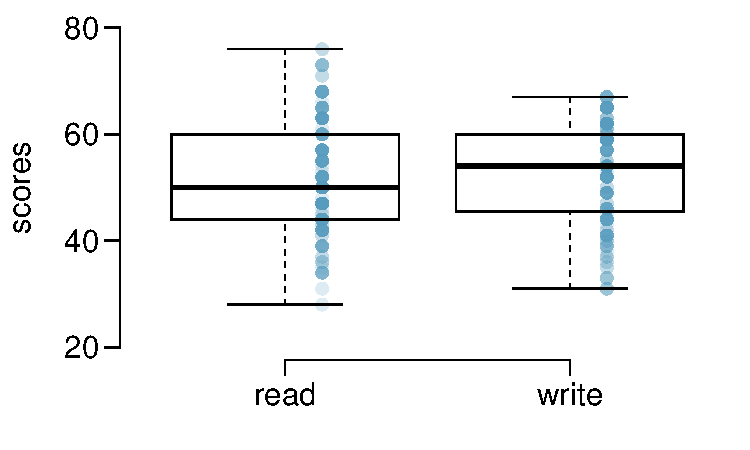
\includegraphics[width=0.5\textwidth]{5-2_paired/figures/hsb2/hsb2_read_write_box}
\end{center}

\end{frame}

%%%%%%%%%%%%%%%%%%%%%%%%%%%%%%%%%%%%

\begin{frame}

\pq{The same students took a reading and writing test and their scores are shown below. Are the reading and writing scores of each student independent of each other?}

{\small
\begin{center}
\begin{tabular}{rrrr}
  \hline
 & id & read & write \\ 
  \hline
1 & 70 & 57 & 52 \\ 
  2 & 86 & 44 & 33 \\ 
  3 & 141 & 63 & 44 \\ 
  4 & 172 & 47 & 52 \\ 
  $\vdots$ &   $\vdots$  &   $\vdots$ &   $\vdots$  \\
  200 & 137 & 63 & 65 \\ 
   \hline
\end{tabular}
\end{center}
}

\begin{multicols}{2}
\begin{enumerate}[(a)]
\item Yes
\solnMult{No}
\end{enumerate}
\end{multicols}

\end{frame}

%%%%%%%%%%%%%%%%%%%%%%%%%%%%%%%%%%%%

\begin{frame}
\frametitle{Analyzing paired data}

\begin{itemize}

\item When two sets of observations have this special correspondence (not independent), they are said to be \hl{paired}.

\pause

\item To analyze paired data, it is often useful to look at the difference in outcomes of each pair of observations. 
\[ \text{diff} = \text{read} - \text{write} \]

\pause

\item It is important that we always subtract using a consistent order.

\end{itemize}

\twocol{0.5}{0.5}{
{\small
\begin{center}
\begin{tabular}{rrrr >{\columncolor[gray]{.9}}r}
  \hline
 & id & read & write & diff \\ 
  \hline
1 & 70 & 57 & 52 & 5 \\ 
  2 & 86 & 44 & 33 & 11 \\ 
  3 & 141 & 63 & 44 & 19 \\ 
  4 & 172 & 47 & 52 & -5 \\ 
  $\vdots$ &   $\vdots$  &   $\vdots$ &   $\vdots$ &   $\vdots$ \\
  200 & 137 & 63 & 65 & -2 \\ 
   \hline
\end{tabular}
\end{center}
}
}
{
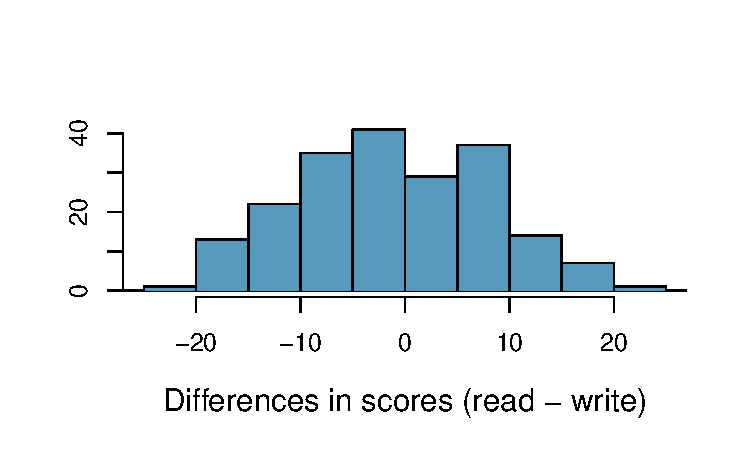
\includegraphics[width=\textwidth]{5-2_paired/figures/hsb2/hsb2_diff_hist}
}

\end{frame}

%%%%%%%%%%%%%%%%%%%%%%%%%%%%%%%%%%%%

\begin{frame}
\frametitle{Parameter and point estimate}

\begin{itemize}

\item \hl{Parameter of interest:} Average difference between the reading and writing scores of \orange{all} high school students.
\[ \mu_{diff} \]

$\:$ \\

\pause

\item \hl{Point estimate:} Average difference between the reading and writing scores of \orange{sampled} high school students.
\[ \bar{x}_{diff} \]

\end{itemize}

\end{frame}

%%%%%%%%%%%%%%%%%%%%%%%%%%%%%%%%%%%%

\subsection{Inference for paired data}

\begin{frame}
\frametitle{Setting the hypotheses}

\dq{If in fact there was no difference between the scores on the reading and writing exams, what would you expect the average difference to be?}

\pause

\soln{0}

$\:$ \\

\pause

\dq{What are the hypotheses for testing if there is a difference between the average reading and writing scores?}

\pause

\begin{itemize}
\item[$H_0$:] There is no difference between the average reading and writing score. 
\[ \mu_{diff} = 0 \]
\item[$H_A$:] There is a difference between the average reading and writing score. 
\[ \mu_{diff} \ne 0 \]
\end{itemize}

\end{frame}

%%%%%%%%%%%%%%%%%%%%%%%%%%%%%%%%%%%%

\begin{frame}
\frametitle{Nothing new here}

\begin{itemize}

\item The analysis is no different than what we have done before.

\item We have data from \orange{one} sample: differences. 

\item We are testing to see if the average difference is different than 0.

\end{itemize}

\end{frame}

%%%%%%%%%%%%%%%%%%%%%%%%%%%%%%%%%%%%

\begin{frame}
\frametitle{Checking assumptions \& conditions}

\pq{Which of the following is true?}

\begin{enumerate}[(a)]
\solnMult{Since students are sampled randomly and are less than 10\% of all high school students, we can assume that the difference between the reading and writing scores of one student in the sample is independent of another.}
\item The distribution of differences is bimodal, therefore we cannot continue with the hypothesis test.
\item In order for differences to be random we should have sampled with replacement.
\item Since students are sampled randomly and are less than 10\% all students, we can assume that the sampling distribution of the average difference will be nearly normal.
\end{enumerate}

\end{frame}

%%%%%%%%%%%%%%%%%%%%%%%%%%%%%%%%%%%

\begin{frame}[shrink]
\frametitle{Calculating the test-statistic and the p-value}

\dq{The observed average difference between the two scores is -0.545 points and the standard deviation of the difference is 8.887 points. Do these data provide convincing evidence of a difference between the average scores on the two exams? Use $\alpha = 0.05$.}

\twocol{0.5}{0.5}
{
\begin{center}
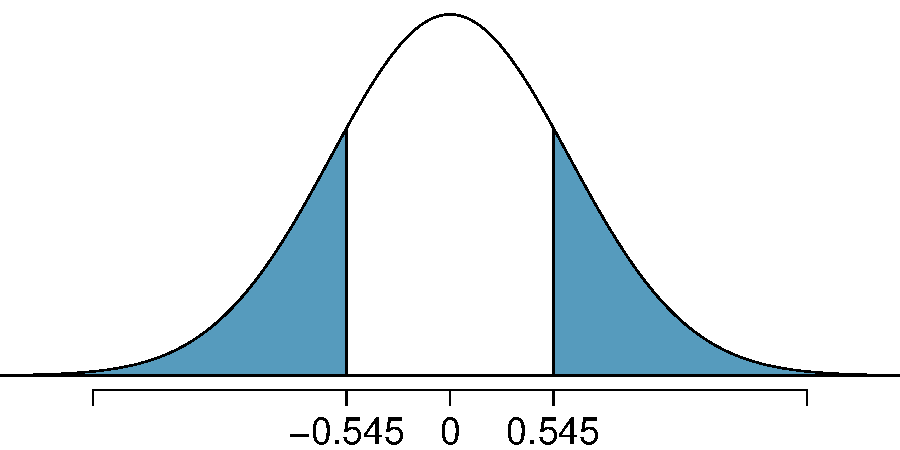
\includegraphics[width=\textwidth]{5-2_paired/figures/hsb2/hsb2_read_write_pval}
\end{center}
}
{
\pause
\begin{eqnarray*}
T &=& \frac{-0.545 - 0}{\frac{8.887}{\sqrt{200}}} \\
&=& \frac{-0.545}{0.628} = -0.87 \\
df &=& 200 - 1 = 199 \\
\pause
p-value &=& 0.1927 \times 2 = 0.3854
\end{eqnarray*}
}
\pause 
$\:$ \\
Since p-value $>$ 0.05, fail to reject, the data do \underline{not} provide convincing evidence of a difference between the average reading and writing scores.

\end{frame}

%%%%%%%%%%%%%%%%%%%%%%%%%%%%%%%%%%%

\begin{frame}
\frametitle{Interpretation of p-value}

\pq{Which of the following is the correct interpretation of the p-value?}

\begin{enumerate}[(a)]
\item Probability that the average scores on the reading and writing exams are equal.
\item Probability that the average scores on the reading and writing exams are different.
\solnMult{Probability of obtaining a random sample of 200 students where the average difference between the reading and writing scores is at least 0.545 (in either direction), if in fact the true average difference between the scores is 0.}
\item Probability of incorrectly rejecting the null hypothesis if in fact the null hypothesis is true.
\end{enumerate}

\end{frame}

%%%%%%%%%%%%%%%%%%%%%%%%%%%%%%%%%%%%

\begin{frame}
\frametitle{HT $\leftrightarrow$ CI}

\pq{Suppose we were to construct a 95\% confidence interval for the average difference between the reading and writing scores. Would you expect this interval to include 0?}

\begin{enumerate}[(a)]
\solnMult{yes}
\item no
\item cannot tell from the information given
\end{enumerate}

\soln{\pause
\begin{eqnarray*} 
-0.545 \pm 1.97 \frac{8.887}{\sqrt{200}} &=& -0.545 \pm 1.97 \times 0.628 \\
&=& -0.545 \pm 1.24 \\
&=& (-1.785, 0.695)
\end{eqnarray*}
}

\end{frame}

%%%%%%%%%%%%%%%%%%%%%%%%%%%%%%%%%%%%
%%%%%%%%%%%%%%%%%%%%%%%%%%%%%%%%%%%%

\section{Difference of two means}

%%%%%%%%%%%%%%%%%%%%%%%%%%%%%%%%%%%%

\begin{frame}
\frametitle{Diamonds}

\begin{itemize}

\item Weights of diamonds are measured in carats. 

\item 1 carat = 100 points, 0.99 carats = 99 points, etc.

\item The difference between the size of a 0.99 carat diamond and a 1 carat diamond is undetectable to the naked human eye, but does the price of a 1 carat diamond tend to be higher than the price of a 0.99 diamond?

\item We are going to test to see if there is a difference between the average prices of 0.99 and 1 carat diamonds.

\item In order to be able to compare equivalent units, we divide the prices of 0.99 carat diamonds by 99 and 1 carat diamonds by 100, and compare the average point prices.

\end{itemize}

\hfill 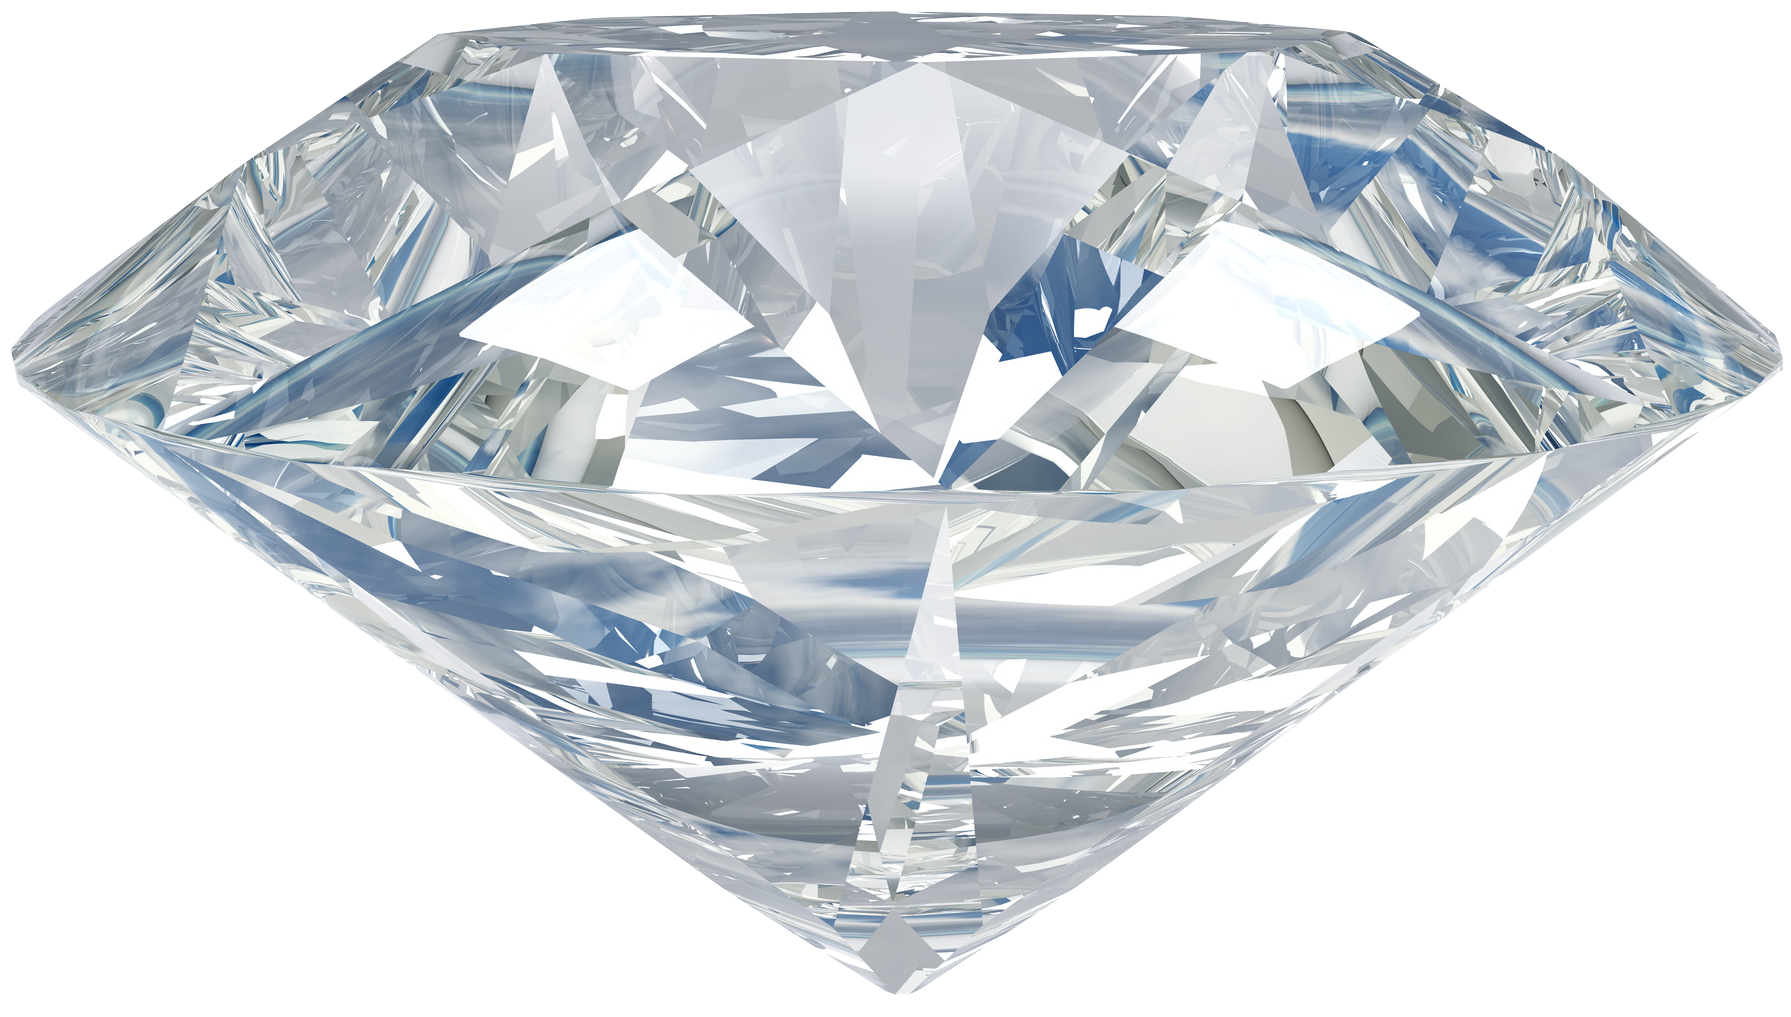
\includegraphics[width=0.3\textwidth]{5-3_diff_two_mean/figures/diamonds/diamond}

\end{frame}

%%%%%%%%%%%%%%%%%%%%%%%%%%%%%%%%%%%

\begin{frame}[fragile]
\frametitle{Data}

\begin{center}
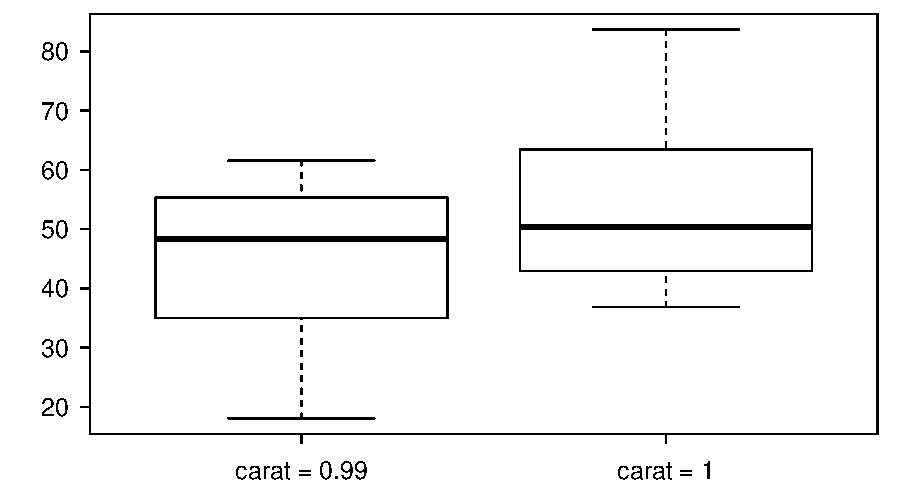
\includegraphics[width=0.7\textwidth]{5-3_diff_two_mean/figures/diamonds/diamondBox}
\end{center}

{\small
\begin{center}
\begin{tabular}{l | c | c}
		& {\footnotesize \hl{0.99 carat}} &  {\footnotesize \hl{1 carat}}  \\
		& pt99	& pt100 \\
\hline
$\bar{x}$	& 44.50		& 53.43 \\
$s$		& 13.32		& 12.22 \\
$n$		& 23			& 30
\end{tabular}
\end{center}
}

\vfill

\rule{2.5cm}{0.25pt} \\
{\tiny These data are a random sample from the \texttt{diamonds} data set in \texttt{ggplot2} R package.}

\end{frame}

%%%%%%%%%%%%%%%%%%%%%%%%%%%%%%%%%%%

\begin{frame}
\frametitle{Parameter and point estimate}

\begin{itemize}

\item \hl{Parameter of interest:} Average difference between the point prices of \orange{all} 0.99 carat and 1 carat diamonds.
\[ \mu_{pt99} - \mu_{pt100} \]

$\:$ \\

\pause

\item \hl{Point estimate:} Average difference between the point prices of \orange{sampled}  0.99 carat and 1 carat diamonds.
\[ \bar{x}_{pt99} - \bar{x}_{pt100} \]

\end{itemize}

\end{frame}

%%%%%%%%%%%%%%%%%%%%%%%%%%%%%%%%%%%

\begin{frame}
\frametitle{Hypotheses}

\pq{Which of the following is the correct set of hypotheses for testing if the average point price of 1 carat diamonds ($_{pt100}$) is higher than the average point price of 0.99 carat diamonds ($_{pt99}$)?}

\begin{enumerate}[(a)]

\item  \mathhl{H_0:} $\mu_{pt99} = \mu_{pt100}$ \\
\mathhl{H_A:} $\mu_{pt99} \ne \mu_{pt100}$

\item  \mathhl{H_0:} $\mu_{pt99} = \mu_{pt100}$ \\
\mathhl{H_A:} $\mu_{pt99} > \mu_{pt100}$

\solnMult{  \mathhl{H_0:} $\mu_{pt99} = \mu_{pt100}$ \\
\mathhl{H_A:} $\mu_{pt99} < \mu_{pt100}$ }

\item  \mathhl{H_0:} $\bar{x}_{pt99} = \bar{x}_{pt100}$ \\
\mathhl{H_A:} $\bar{x}_{pt99} < \bar{x}_{pt100}$

\end{enumerate}

\end{frame}

%%%%%%%%%%%%%%%%%%%%%%%%%%%%%%%%%%%

\begin{frame}
\frametitle{Conditions}

\pq{Which of the following does \underline{not} need to be satisfied in order to conduct this hypothesis test using theoretical methods?}

\begin{enumerate}[(a)]

\item Point price of one 0.99 carat diamond in the sample should be independent of another, and the point price of one 1 carat diamond should independent of another as well.

\item Point prices of 0.99 carat and 1 carat diamonds in the sample should be independent.

\item Distributions of point prices of 0.99 and 1 carat diamonds should not be extremely skewed.

\solnMult{Both sample sizes should be at least 30.}

\end{enumerate}

\end{frame}

%%%%%%%%%%%%%%%%%%%%%%%%%%%%%%%%%%%%

\subsection{Sampling distribution for the difference of two means}

%%%%%%%%%%%%%%%%%%%%%%%%%%%%%%%%%%%%

\begin{frame}
\frametitle{Test statistic}

\formula{Test statistic for inference on the difference of two small sample means}
{The test statistic for inference on the difference of two means where $\sigma_1$ and $\sigma_2$ are unknown is the $T$ statistic.
\[ T_{df} = \frac{\text{point estimate} - \text{null value}}{SE} \]
where 
\[ SE = \sqrt{ \frac{s_1^2}{n_1} + \frac{s_2^2}{n_2} } \qquad \text{ and } \qquad df = min(n_1 - 1, n_2 - 1) \]
}

\Note{The calculation of the $df$ is actually much more complicated. For simplicity we'll use the above formula to \underline{estimate} the true $df$ when conducting the analysis by hand.}

\end{frame}

%%%%%%%%%%%%%%%%%%%%%%%%%%%%%%%%%%%%

\subsection{Hypothesis testing for the difference of two means}

%%%%%%%%%%%%%%%%%%%%%%%%%%%%%%%%%%%%

\begin{frame}
\frametitle{Test statistic (cont.)}

{\small
\begin{center}
\begin{tabular}{l | c | c}
		& {\footnotesize \hl{0.99 carat}} &  {\footnotesize \hl{1 carat}}  \\
		& pt99	& pt100 \\
\hline
$\bar{x}$	& 44.50		& 53.43 \\
$s$		& 13.32		& 12.22 \\
$n$		& 23			& 30
\end{tabular}
\end{center}
}

\hl{in context...}

\pause

{\small
\begin{eqnarray*}
T &=& \frac{\text{point estimate} - \text{null value} }{SE} \\
\pause
&=& \frac{(44.50 - 53.43) - 0}{ \sqrt{\frac{13.32^2}{23} + \frac{12.22^2}{30} }} \\
\pause
&=& \frac{-8.93}{3.56} \\
\pause
&=& -2.508
\end{eqnarray*}
}

\end{frame}

%%%%%%%%%%%%%%%%%%%%%%%%%%%%%%%%%%%%

\begin{frame}
\frametitle{Test statistic (cont.)}

\pq{Which of the following is the correct $df$ for this hypothesis test?}

\twocol{0.3}{0.7}
{
\begin{enumerate}[(a)]
\solnMult{ 22 }
\item 23
\item 30
\item 29
\item 52
\end{enumerate}
}
{
\soln{\only<2>{
\orange{$\rightarrow df = min(n_{pt99} - 1, n_{pt100} - 1)$ \\
$= min(23 - 1, 30 - 1)$ \\
$= min(22,29) = 22$} \\
\vspace{1cm}
}}}

\end{frame}

%%%%%%%%%%%%%%%%%%%%%%%%%%%%%%%%%%%%

\begin{frame}
\frametitle{p-value}

\pq{Which of the following is the correct p-value for this hypothesis test?}

\[ T = -2.508 \qquad \only<1-2 | handout:0>{df = 22} \] 

\twocol{0.42}{0.58}
{
\begin{enumerate}[(a)]
\item between 0.005 and 0.01
\solnMult{between 0.01 and 0.025}
\item between 0.02 and 0.05
\item between 0.01 and 0.02
\end{enumerate}
}
{
\only<1>{
{\footnotesize
\begin{tabular}{r | r r  r r r}
\hline
one tail & \hspace{1.5mm}  0.100 & \hspace{1.5mm} 0.050 & \hspace{1.5mm} {0.025} & \hspace{1.5mm} {0.010} & \hspace{1.5mm} 0.005  \\
two tails & 0.200 & 0.100 & 0.050 & 0.020 & 0.010 \\
\hline
df \hfill 21  &  {  1.32} & {  1.72} & {  2.08} & {  2.52} & {  2.83}  \\ 
22  &  {  1.32} & {  1.72} & {  2.07} & {  2.51} & {  2.82}  \\ 
23  &  {  1.32} & {  1.71} & {  2.07} & {  2.50} & {  2.81}  \\ 
24  &  {  1.32} & {  1.71} & {  2.06} & {  2.49} & {  2.80}  \\ 
25  &  {  1.32} & {  1.71} & {  2.06} & {  2.49} & {  2.79}  \\ 
\hline
\end{tabular}
}
}

\only<2|handout:0>{
{\footnotesize
\begin{tabular}{r | r r  >{\columncolor[gray]{.6}[.5\tabcolsep]}r  >{\columncolor[gray]{.6}[.5\tabcolsep]}r r}
\hline
one tail & \hspace{1.5mm}  0.100 & \hspace{1.5mm} 0.050 & \hspace{1.5mm} \orange{0.025} & \hspace{1.5mm} \orange{0.010} & \hspace{1.5mm} 0.005  \\
two tails & 0.200 & 0.100 & 0.050 & 0.020 & 0.010 \\
\hline
df \hfill 21  &  {  1.32} & {  1.72} & {  2.08} & {  2.52} & {  2.83}  \\ 
  \rowcolor[gray]{.6}
22  &  {  1.32} & {  1.72} & \orange{  2.07} & \orange{  2.51} & {  2.82}  \\ 
23  &  {  1.32} & {  1.71} & {  2.07} & {  2.50} & {  2.81}  \\ 
24  &  {  1.32} & {  1.71} & {  2.06} & {  2.49} & {  2.80}  \\ 
25  &  {  1.32} & {  1.71} & {  2.06} & {  2.49} & {  2.79}  \\ 
\hline
\end{tabular}
}
}}

\end{frame}

%%%%%%%%%%%%%%%%%%%%%%%%%%%%%%%%%%%%

\begin{frame}
\frametitle{Synthesis}

\dq{What is the conclusion of the hypothesis test? How (if at all) would this conclusion change your behavior if you went diamond shopping?}


\soln{\only<2>{
\begin{itemize}
\item p-value is small so reject $H_0$. The data provide convincing evidence to suggest that the point price of 0.99 carat diamonds is lower than the point price of 1 carat diamonds.
\item Maybe buy a 0.99 carat diamond? It looks like a 1 carat, but is significantly cheaper.
\end{itemize}
}}

\end{frame}

%%%%%%%%%%%%%%%%%%%%%%%%%%%%%%%%%%%%

\subsection{Confidence intervals for the difference of two means}

%%%%%%%%%%%%%%%%%%%%%%%%%%%%%%%%%%%%

\begin{frame}
\frametitle{Equivalent confidence level}

\pq{What is the equivalent confidence level for a one-sided hypothesis test at $\alpha = 0.05$?}


\twocol{0.3}{0.7}{
\begin{enumerate}[(a)]

\solnMult{90\%}

\item 92.5\%

\item 95\%

\item 97.5\%

\end{enumerate}
}
{
\soln{\only<2>{
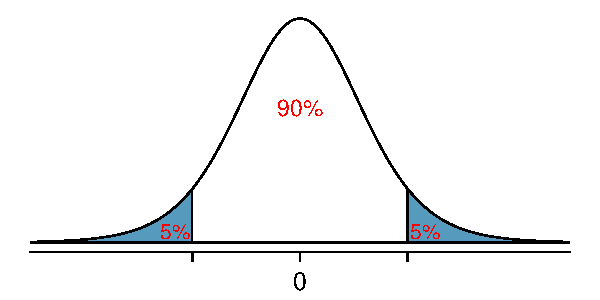
\includegraphics[width=\textwidth]{5-3_diff_two_mean/figures/middle90/middle90}
}}
}

\end{frame}

%%%%%%%%%%%%%%%%%%%%%%%%%%%%%%%%%%%%

\begin{frame}
\frametitle{Critical value}

\pq{What is the appropriate $t^\star$ for a confidence interval for the average difference between the point prices of 0.99 and 1 carat diamonds?}

\begin{enumerate}[(a)]
\item 1.32
\solnMult{1.72}
\item 2.07
\item 2.82
\end{enumerate}

\only<1>{
{\small
\begin{center}
\begin{tabular}{r | r r r r r}
\hline
one tail & \hspace{1.5mm}  0.100 & \hspace{1.5mm} {0.050} & \hspace{1.5mm} {0.025} & \hspace{1.5mm} {0.010} & \hspace{1.5mm} 0.005  \\
two tails & 0.200 & 0.100 & 0.050 & 0.020 & 0.010 \\
\hline
df \hfill 21  &  {  1.32} & {  1.72} & {  2.08} & {  2.52} & {  2.83}  \\ 
22  &  {  1.32} & {  1.72} & {  2.07} & {  2.51} & {  2.82}  \\ 
23  &  {  1.32} & {  1.71} & {  2.07} & {  2.50} & {  2.81}  \\ 
24  &  {  1.32} & {  1.71} & {  2.06} & {  2.49} & {  2.80}  \\ 
25  &  {  1.32} & {  1.71} & {  2.06} & {  2.49} & {  2.79}  \\ 
\end{tabular}
\end{center}
}}

\only<2|handout:0>{
\begin{center}
{\small
\begin{tabular}{r | r >{\columncolor[gray]{.6}[.5\tabcolsep]}r r  r r}
\hline
one tail & \hspace{1.5mm}  0.100 & \hspace{1.5mm} {0.050} & \hspace{1.5mm} {0.025} & \hspace{1.5mm} {0.010} & \hspace{1.5mm} 0.005  \\
two tails & 0.200 & \orange{0.100} & 0.050 & 0.020 & 0.010 \\
\hline
df \hfill 21  &  {  1.32} & {  1.72} & {  2.08} & {  2.52} & {  2.83}  \\ 
  \rowcolor[gray]{.6}
22  &  {  1.32} & \orange{  1.72} & {  2.07} & {  2.51} & {  2.82}  \\ 
23  &  {  1.32} & {  1.71} & {  2.07} & {  2.50} & {  2.81}  \\ 
24  &  {  1.32} & {  1.71} & {  2.06} & {  2.49} & {  2.80}  \\ 
25  &  {  1.32} & {  1.71} & {  2.06} & {  2.49} & {  2.79}  \\ 
\hline
\end{tabular}
}
\end{center}
}


\end{frame}

%%%%%%%%%%%%%%%%%%%%%%%%%%%%%%%%%%%%

\begin{frame}
\frametitle{Confidence interval}

\dq{Calculate the interval, and interpret it in context.}

\pause

\soln{
\[ \text{point estimate} \pm ME \]
\pause
\begin{eqnarray*}
(\bar{x}_{pt99} - \bar{x}_{pt1}) \pm t^\star_{df} \times SE &=& (44.50 - 53.43) \pm 1.72 \times 3.56 \\
\pause
&=& -8.93 \pm  6.12 \\
\pause
&=& (-15.05, -2.81)
\end{eqnarray*}
\pause
We are 90\% confident that the average point price of a 0.99 carat diamond is \$15.05 to \$2.81 lower than the average point price of a 1 carat diamond.
}

\end{frame}

%%%%%%%%%%%%%%%%%%%%%%%%%%%%%%%%%%%%

\subsection{Recap}

%%%%%%%%%%%%%%%%%%%%%%%%%%%%%%%%%%%%

\begin{frame}
\frametitle{Recap: Inference using difference of two small sample means}

\begin{itemize}

\item If $\sigma_1$ or $\sigma_2$ is unknown, difference between the sample means follow a $t$-distribution with $SE = \sqrt{ \frac{s_1^2}{n_1} + \frac{s_2^2}{n_1} }$.

\pause

\item Conditions: 
\begin{itemize}
\item independence within groups (often verified by a random sample, and if sampling without replacement, $n < $ 10\% of population) and between groups
\item no extreme skew in either group
\end{itemize}

\pause

\item Hypothesis testing: 
\[ T_{df} = \frac{\text{point estimate} - \text{null value}}{SE}\text{, where }df = min(n_1 - 1, n_2 - 1) \]

\pause

\item Confidence interval:
\[ \text{point estimate} \pm t_{df}^\star \times SE \]

\end{itemize}

\end{frame}

%%%%%%%%%%%%%%%%%%%%%%%%%%%%%%%%%%%
%%%%%%%%%%%%%%%%%%%%%%%%%%%%%%%%%%%%

\section{Computing the power for a 2-sample test}

%%%%%%%%%%%%%%%%%%%%%%%%%%%%%%%%%%%%

\begin{frame}
\frametitle{}

\begin{center}
\begin{tabular}{l l | c c}
\multicolumn{2}{c}{} & \multicolumn{2}{c}{\textbf{Decision}} \\
& & fail to reject $H_0$ &  reject $H_0$ \\
  \cline{2-4}
& $H_0$ true & \onslide<4->{\green{$1 - \alpha$}} & \onslide<2->{\orange{Type 1 Error, $\alpha$}} \\
\raisebox{1.5ex}{\textbf{Truth}} & $H_A$ true &  \onslide<3->{\orange{Type 2 Error, $\beta$}} & \onslide<5->{\green{Power, $1 - \beta$}} \\
  \cline{2-4}
\end{tabular}
\end{center}

\pause

\begin{itemize}
\item Type 1 error is rejecting $H_0$ when you shouldn't have, and the probability of doing so is $\alpha$ (significance level)

\pause 

\item Type 2 error is failing to reject $H_0$ when you should have, and the probability of doing so is $\beta$ (a little more complicated to calculate)

\pause 

\item \hl{Power} of a test is the probability of correctly rejecting $H_0$, and the probability of doing so is $1 - \beta$

\pause 

\item In hypothesis testing, we want to keep $\alpha$ and $\beta$ low, but there are inherent trade-offs.

\end{itemize}

\end{frame}

%%%%%%%%%%%%%%%%%%%%%%%%%%%%%%%%%%%%

\begin{frame}
\frametitle{Type 2 error rate}

If the alternative hypothesis is actually true, what is the chance that we make a Type 2 Error, i.e. we fail to reject the null hypothesis even when we should reject it?

\begin{itemize}

\item The answer is not obvious.

\item If the true population average is very close to the null hypothesis value, it will be difficult to detect a difference (and reject $H_0$).

\item If the true population average is very different from the null hypothesis value, it will be easier to detect a difference.

\item Clearly, $\beta$ depends on the \hl{effect size} ($\delta$)
\end{itemize}

\end{frame}

%%%%%%%%%%%%%%%%%%%%%%%%%%%%%%%%%%%%

\begin{frame}
\frametitle{Example - Blood Pressure (BP), hypotheses}

{\dq
{\footnotesize
Suppose a pharmaceutical company has developed a new drug for lowering blood pressure, and they are preparing a clinical trial to test the drug's effectiveness. They recruit people who are taking a particular standard blood pressure medication, and half of the subjects are given the new drug (treatment) and the other half continue to take their current medication through generic-looking pills to ensure blinding (control). What are the hypotheses for a two-sided hypothesis test in this context?
}
}

\pause

\soln{
\begin{align*}
H_0&: \mu_{treatment} - \mu_{control} = 0 \\
H_A&: \mu_{treatment} - \mu_{control} \ne 0  
\end{align*}
}

\end{frame}

%%%%%%%%%%%%%%%%%%%%%%%%%%%%%%%%%%%%

\begin{frame}
\frametitle{Example - BP, standard error}

{\dq
{\footnotesize
Suppose researchers would like to run the clinical trial on patients with systolic blood pressures between 140 and 180 mmHg. Suppose previously published studies suggest that the standard deviation of the patients' blood pressures will be about 12 mmHg and the distribution of patient blood pressures will be approximately symmetric. If we had 100 patients per group, what would be the approximate standard error for difference in sample means of the treatment and control groups?
}
}

\pause

\soln{
\[ SE = \sqrt{ \frac{12^2}{100} + \frac{12^2}{100} } = 1.70 \]
}

\end{frame}

%%%%%%%%%%%%%%%%%%%%%%%%%%%%%%%%%%%%

\begin{frame}
\frametitle{Example - BP, minimum effect size required to reject $H_0$}

{\dq
{\footnotesize
For what values of the difference between the observed averages of blood pressure in treatment and control groups (effect size) would we reject the null hypothesis at the 5\% significance level?}
}

\pause

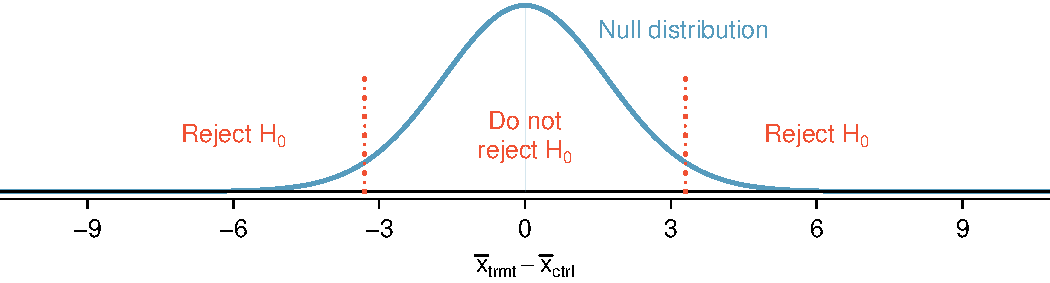
\includegraphics[width=\textwidth]{5-4_power/figures/power/power_null_B_0_1-7_with_rejection_region}

\pause

The difference should be at least 
\[ 1.96 * 1.70 = 3.332 \] 
or at most 
\[ -1.96 * 1.70 = 3.332. \]

\end{frame}

%%%%%%%%%%%%%%%%%%%%%%%%%%%%%%%%%%%%

\begin{frame}
\frametitle{Example - BP, power}

{\dq
{\footnotesize
Suppose that the company researchers care about finding any effect on blood pressure that is 3 mmHg or larger vs the standard medication. What is the power of the test that can detect this effect?
}}

\pause

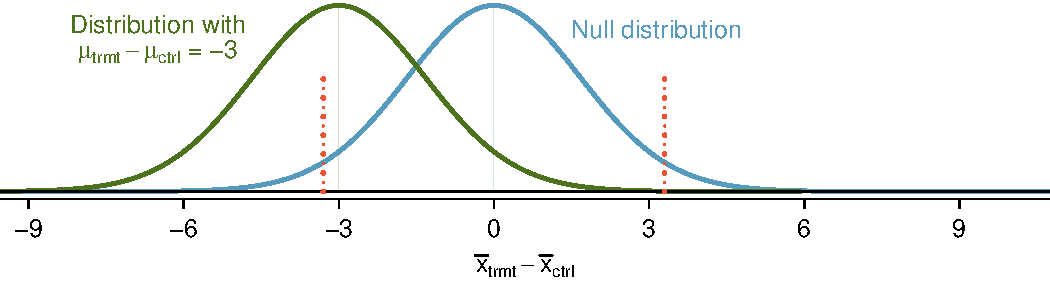
\includegraphics[width=\textwidth]{5-4_power/figures/power/power_null_C_0_1-7_with_alt_at_3}

\pause

\[ Z = \frac{-3.332 - (-3)}{1.70} = -0.20 \]

\pause

\[ P(Z < -0.20) = 0.4207 \]

\end{frame}

%%%%%%%%%%%%%%%%%%%%%%%%%%%%%%%%%%%%

\begin{frame}
\frametitle{Example - BP, required sample size for 80\% power}

{\dq
{\footnotesize
What sample size will lead to a power of 80\% for this test?
}}

\pause

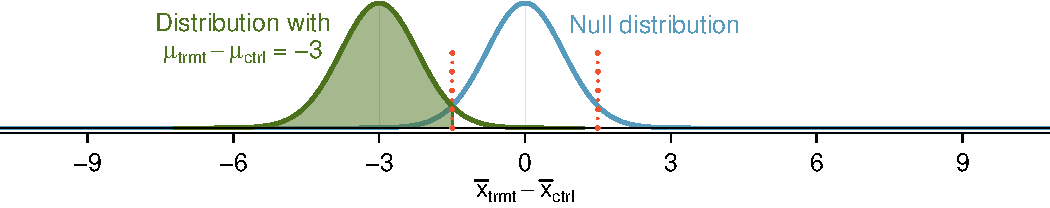
\includegraphics[width=\textwidth]{5-4_power/figures/power/power_null_0_0-76_with_alt_at_3_and_shaded}

\pause

\[ SE = \frac{3}{2.8} = 1.07142 \]

\pause

\[ 1.07142 = \sqrt{ \frac{12^2}{n} + \frac{12^2}{n} } \]

\pause

\[ n = 250.88 \rightarrow n \ge 251 \]

\end{frame}

%%%%%%%%%%%%%%%%%%%%%%%%%%%%%%%%%%%%

\begin{frame}
\frametitle{Recap}

\begin{itemize}
\item Calculate required sample size for a desired level of power
\item Calculate power for a range of sample sizes, then choose the sample size that yields the target power (usually 80\% or 90\%)
\end{itemize}
\begin{center}
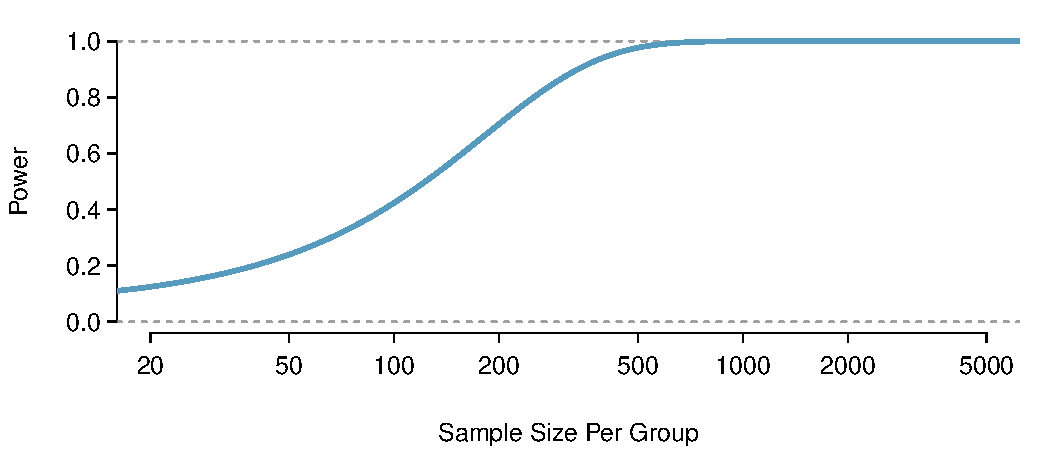
\includegraphics[width=0.7\textwidth]{5-4_power/figures/power/power_curve_neg-3}
\end{center}

\end{frame}

%%%%%%%%%%%%%%%%%%%%%%%%%%%%%%%%%%%%

\begin{frame}
\frametitle{Achieving desired power}

There are several ways to increase power (and hence decrease type 2 error rate):

\pause

{\small
\begin{enumerate}

\item Increase the sample size.

\pause

\item Decrease the standard deviation of the sample, which essentially has the same effect as increasing the sample size (it will decrease the standard error). With a smaller $s$ we have a better chance of distinguishing the null value from the observed point estimate. This is difficult to ensure but cautious measurement process and limiting the population so that it is more homogenous may help.

\pause

\item Increase $\alpha$, which will make it more likely to reject $H_0$ (but note that this has the side effect of increasing the Type 1 error rate).

\pause

\item Consider a larger effect size. If the true mean of the population is in the alternative hypothesis but close to the null value, it will be harder to detect a difference.

\end{enumerate}
}

\end{frame}

%%%%%%%%%%%%%%%%%%%%%%%%%%%%%%%%%%%%
%%%%%%%%%%%%%%%%%%%%%%%%%%%%%%%%%%

\section{Comparing means with ANOVA}

%%%%%%%%%%%%%%%%%%%%%%%%%%%%%%%%%%%

\subsection{Aldrin in the Wolf River}

%%%%%%%%%%%%%%%%%%%%%%%%%%%%%%%%%%%

\begin{frame}
\frametitle{}

\begin{center}
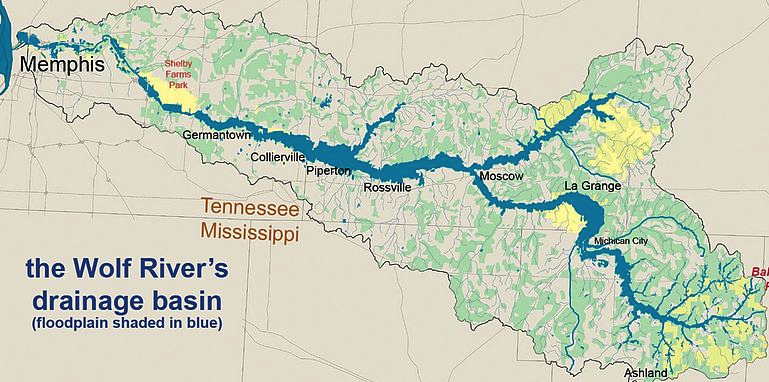
\includegraphics[width=0.6\textwidth]{5-5_anova/figures/aldrin/wolf}
\end{center}

{\small
\begin{itemize}

\item  The Wolf River in Tennessee flows past an abandoned site once used by the pesticide industry for dumping wastes, including chlordane (pesticide), aldrin, and dieldrin (both insecticides).

\pause

\item These highly toxic organic compounds can cause various cancers and birth defects.

\pause

\item The standard methods to test whether these substances are present in a river is to take samples at six-tenths depth. 

\pause

\item But since these compounds are denser than water and their molecules tend to stick to particles of sediment, they are more likely to be found in higher concentrations near the bottom than near mid-depth.

\end{itemize}
}

\end{frame}

%%%%%%%%%%%%%%%%%%%%%%%%%%%%%%%%%%%

\begin{frame}
\frametitle{Data}

Aldrin concentration (nanograms per liter) at three levels of depth. \\

\begin{center}
\begin{tabular}{r | c | c}
\hline
 	& aldrin 					& depth \\ 
\hline
1 	& \textcolor{darkGray}{3.80} 	& \textcolor{darkGray}{bottom}  \\ 
2 	& \textcolor{darkGray}{4.80} 	& \textcolor{darkGray}{bottom}  \\ 
...	&						& \\
10	& \textcolor{darkGray}{8.80} 	& \textcolor{darkGray}{bottom} \\
11	& \textcolor{blue}{3.20} 		& \textcolor{blue}{middepth}  \\
12	& \textcolor{blue}{3.80} 		& \textcolor{blue}{middepth} \\
...	&						& \\
20 	& \textcolor{blue}{6.60} 		& \textcolor{blue}{middepth} \\
21	& \textcolor{oiB}{3.10} 		& \textcolor{oiB}{surface} \\
22	& \textcolor{oiB}{3.60} 		& \textcolor{oiB}{surface} \\
...	&						& \\
30 	& \textcolor{oiB}{5.20} 		& \textcolor{oiB}{surface} \\  
\hline
\end{tabular}
\end{center}

\end{frame}

%%%%%%%%%%%%%%%%%%%%%%%%%%%%%%%%%%%

\begin{frame}
\frametitle{Exploratory analysis}

Aldrin concentration (nanograms per liter) at three levels of depth. \\

\begin{center}
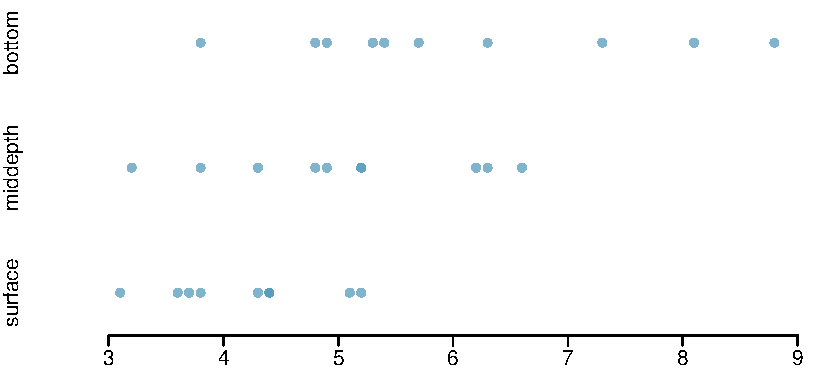
\includegraphics[width=0.75\textwidth]{5-5_anova/figures/aldrin/dotplot}
\end{center}

\begin{center}
\begin{tabular}{l | c c c}
		& n	& mean	& sd		\\
\hline
bottom	& 10	& 6.04	& 1.58 \\
middepth& 10	& 5.05	& 1.10 \\
surface	& 10	& 4.20	& 0.66 \\
\hline
overall	& 30	& 5.1	0	& 1.37
\end{tabular}
\end{center}

\end{frame}

%%%%%%%%%%%%%%%%%%%%%%%%%%%%%%%%%%%

\begin{frame}
\frametitle{Research question}

\dq{Is there a difference between the mean aldrin concentrations among the three levels?}

\vspace{0.5cm}

\pause

\begin{itemize}

\item To compare means of 2 groups we use a Z or a T statistic.

\pause

\item To compare means of 3+ groups we use a new test called \hl{ANOVA} and a new statistic called \hl{F}.

\end{itemize}

\end{frame}

%%%%%%%%%%%%%%%%%%%%%%%%%%%%%%%%%%%

\begin{frame}
\frametitle{ANOVA}

ANOVA is used to assess whether the mean of the outcome variable is different for different levels of a categorical variable.

\pause

\begin{itemize}
\item[] \mathhl{H_0:} The mean outcome is the same across all categories, 
\[\mu_1 = \mu_2 = \cdots = \mu_k, \]
where $\mu_i$ represents the mean of the outcome for observations in category $i$.
\item[]
\item[] \mathhl{H_A:} At least one mean is different than others.
\end{itemize}

\end{frame}

%%%%%%%%%%%%%%%%%%%%%%%%%%%%%%%%%%%

\begin{frame}
\frametitle{Conditions}

\begin{enumerate}

\item The observations should be independent within and between groups

\begin{itemize}
\item If the data are a simple random sample from less than 10\% of the population, this condition is satisfied.
\item Carefully consider whether the data may be independent (e.g. no pairing). 
\item Always important, but sometimes difficult to check.
\end{itemize}

\pause

\item The observations within each group should be nearly normal.

\begin{itemize}
\item Especially important when the sample sizes are small.
\end{itemize}

\dq{How do we check for normality?}

\pause

\item The variability across the groups should be about equal.

\begin{itemize}
\item Especially important when the sample sizes differ between groups.
\end{itemize}

\dq{How can we check this condition?}

\end{enumerate}

\end{frame}

%%%%%%%%%%%%%%%%%%%%%%%%%%%%%%%%%%%

\begin{frame}
\frametitle{$z$/$t$ test vs. ANOVA - Purpose}

\twocol{0.5}{0.5}
{
\[ \hl{$z$/$t$ test} \]
Compare means from \hl{two} groups to see whether they are so far apart that the observed difference cannot reasonably be attributed to sampling variability.
\[ H_0: \mu_1 = \mu_2 \]
}
{
\[ \hl{ANOVA} \]
Compare the means from \hl{two or more} groups to see whether they are so far apart that the observed differences cannot all reasonably be attributed to sampling variability.
\[ H_0: \mu_1 = \mu_2 = \cdots = \mu_k \]
}

\end{frame}

%%%%%%%%%%%%%%%%%%%%%%%%%%%%%%%%%%%

\begin{frame}
\frametitle{$z$/$t$ test vs. ANOVA - Method}

\twocol{0.5}{0.5}
{
\[ \hl{$z$/$t$ test} \]
Compute a test statistic (a ratio).
\[ z / t = \frac{(\bar{x}_1 - \bar{x}_2) - (\mu_1 - \mu_2)}{SE(\bar{x}_1 - \bar{x}_2)} \]
}
{
\[ \hl{ANOVA} \]
Compute a test statistic (a ratio).
\[ F = \frac{\text{variability bet. groups}}{\text{variability w/in groups}} \]
}

\vspace{1cm}

\pause

\begin{itemize}

\item Large test statistics lead to small p-values. 

\item If the p-value is small enough $H_0$ is rejected, we conclude that the population means are not equal.

\end{itemize}

\end{frame}

%%%%%%%%%%%%%%%%%%%%%%%%%%%%%%%%%%%

\begin{frame}
\frametitle{$z$/$t$ test vs. ANOVA}

\begin{itemize}

\item With only two groups t-test and ANOVA are equivalent, but only if we use a pooled standard variance in the denominator of the test statistic.

\pause

\item With more than two groups, ANOVA compares the sample means to an overall \hl{grand mean}.

\end{itemize}

\end{frame}

%%%%%%%%%%%%%%%%%%%%%%%%%%%%%%%%%%%

\begin{frame}
\frametitle{Hypotheses}

\pq{What are the correct hypotheses for testing for a difference between the mean aldrin concentrations among the three levels?}

\begin{enumerate}[(a)]
\item $H_0: \mu_B = \mu_M = \mu_S$ \\
$H_A: \mu_B \ne \mu_M \ne \mu_S$ \\
\item $H_0: \mu_B \ne \mu_ M \ne \mu_S$ \\
$H_A: \mu_B = \mu_M = \mu_S$ \\
\solnMult{$H_0: \mu_B = \mu_M = \mu_S$ \\
$H_A:$ At least one mean is different.}
\item $H_0: \mu_B = \mu_M = \mu_S = 0$ \\
$H_A:$ At least one mean is different.
\item $H_0: \mu_B = \mu_M = \mu_S$ \\
$H_A: \mu_B > \mu_M > \mu_S$ \\
\end{enumerate}

\end{frame}

%%%%%%%%%%%%%%%%%%%%%%%%%%%%%%%%%%%

\subsection{ANOVA and the F test}

%%%%%%%%%%%%%%%%%%%%%%%%%%%%%%%%%%%

\begin{frame}
\frametitle{Test statistic}

\dq{Does there appear to be a lot of variability within groups? How about between groups?}

\[ F = \frac{\text{variability bet. groups}}{\text{variability w/in groups}}  \]

\begin{center}
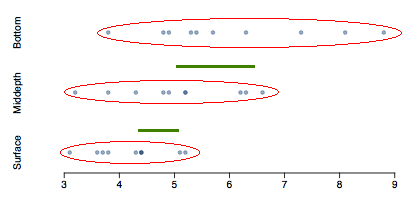
\includegraphics[width=0.75\textwidth]{5-5_anova/figures/aldrin/dotplot_var}
\end{center}

\end{frame}

%%%%%%%%%%%%%%%%%%%%%%%%%%%%%%%%%%%

%\begin{frame}
%\frametitle{Test statistic (cont.)}
%
%\[ F = \frac{\text{variability bet. groups}}{\text{variability w/in groups}} = \frac{\hl{MSG}}{\hl{MSE}}  \]
%
%\begin{itemize}
%
%\item \hl{MSG} is mean square between groups
%\[ df_G = k - 1 \]
%where $k$ is number of groups
%
%\item \hl{MSE} is mean square error - variability in residuals
%\[ df_E = n - k \]
%where $n$ is number of observations.
%
%\end{itemize}
%
%\end{frame}
%
%%%%%%%%%%%%%%%%%%%%%%%%%%%%%%%%%%%%

\begin{frame}
\frametitle{$F$ distribution and p-value}

\[ F =  \frac{\text{variability bet. groups}}{\text{variability w/in groups}} \]

\vspace{-1cm}

\begin{center}
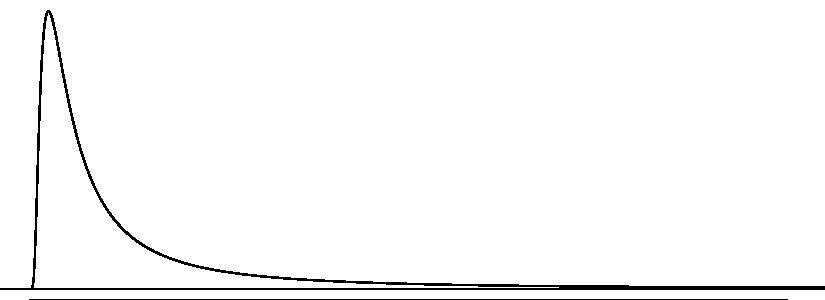
\includegraphics[width=0.75\textwidth]{5-5_anova/figures/fdist/fdist}
\end{center}

\begin{itemize}

\item In order to be able to reject $H_0$, we need a small p-value, which requires a large F statistic.

\item In order to obtain a large F statistic, variability between sample means needs to be greater than variability within sample means.

\end{itemize}

\end{frame}

%%%%%%%%%%%%%%%%%%%%%%%%%%%%%%%%%%%

\subsection{ANOVA output, deconstructed}

%%%%%%%%%%%%%%%%%%%%%%%%%%%%%%%%%%%

\begin{frame}
\frametitle{}

\vspace{-0.5cm}

{\footnotesize
\begin{center}
\begin{tabular}{ll >{\columncolor[gray]{.6}[.5\tabcolsep]}rrrrr}
\hline
 			& 			& Df 	& Sum Sq	& Mean Sq 	& F value 	& Pr($>$F) \\ 
\hline
(\hl{G}roup) 	& depth 		& 2 	& 16.96 	& 8.48 		& 6.13 	& 0.0063 \\ 
(\hl{E}rror) 	& Residuals 	& 27 	& 37.33 	& 1.38 		&  		&  \\ 
\hline
	 		& \hl{T}otal	& 29	& 54.29 \\
\end{tabular}
\end{center}
}

\formula{Degrees of freedom associated with ANOVA}
{
\begin{itemize}
\item groups: $df_G = k - 1$, where $k$ is the number of groups
\item total: $df_T = n - 1$, where $n$ is the total sample size
\item error: $df_E = df_T - df_G$
\end{itemize}
}

\pause

\begin{itemize}

\item $df_G = k - 1 = 3 - 1 = 2$ \\ 

\pause

\item $df_T = n - 1 = 30 - 1 = 29$

\pause

\item $df_E = 29 - 2 = 27$ \\

\end{itemize}

\end{frame}

%%%%%%%%%%%%%%%%%%%%%%%%%%%%%%%%%%%

\begin{frame}
\frametitle{}

\vspace{-0.25cm}

{\footnotesize
\begin{center}
\begin{tabular}{ll r>{\columncolor[gray]{.6}[.5\tabcolsep]}rrrr}
\hline
 			& 			& Df 	& Sum Sq	& Mean Sq 	& F value 	& Pr($>$F) \\ 
\hline
(\hl{G}roup) 	& depth 		& 2 	& \red{16.96} 	& 8.48 		& 6.13 	& 0.0063 \\ 
(\hl{E}rror) 	& Residuals 	& 27 	& 37.33 	& 1.38 		&  		&  \\ 
\hline
	 		& \hl{T}otal	& 29	& 54.29 \\
\end{tabular}
\end{center}
}

\formula{Sum of squares between groups, SSG}
{
Measures the variability between groups 
\vspace{-0.25cm}
\[ SSG = \sum_{i = 1}^{k} n_i (\bar{x}_i - \bar{x})^2 \]
where $n_i$ is each group size, $\bar{x}_i$ is the average for each group, $\bar{x}$ is the overall (grand) mean.
}

\pause

\vspace{-0.5cm}

\twocol{0.4}{0.5}
{
{\small
\begin{center}
\begin{tabular}{l | c c }
		& n	& mean		\\
\hline
bottom	& 10	& 6.04	 \\
middepth& 10	& 5.05	 \\
surface	& 10	& 4.2	 \\
\hline
overall	& 30	& 5.1	
\end{tabular}
\end{center}
}
}
{
\pause
\begin{eqnarray*}
SSG &=& \pr{ 10 \times (6.04 - 5.1)^2 } \\
\pause
&+& \pr{ 10 \times (5.05 - 5.1)^2 } \\
\pause
&+& \pr{ 10 \times (4.2 - 5.1)^2 } \\
\pause
&=& 16.96 \\
\end{eqnarray*}
}

\end{frame}

%%%%%%%%%%%%%%%%%%%%%%%%%%%%%%%%%%%

\begin{frame}
\frametitle{}

\vspace{-0.25cm}

{\footnotesize
\begin{center}
\begin{tabular}{ll r>{\columncolor[gray]{.6}[.5\tabcolsep]}rrrr}
\hline
 			& 			& Df 	& Sum Sq	& Mean Sq 	& F value 	& Pr($>$F) \\ 
\hline
(\hl{G}roup) 	& depth 		& 2 	& 16.96	& 8.48 		& 6.13 	& 0.0063 \\ 
(\hl{E}rror) 	& Residuals 	& 27 	& 37.33 	& 1.38 		&  		&  \\ 
\hline
	 		& \hl{T}otal	& 29	& \red{54.29} \\
\end{tabular}
\end{center}
}

\formula{Sum of squares total, SST}
{
Measures the variability between groups 
\vspace{-0.25cm}
\[ SST = \sum_{i = 1}^{n} (x_i - \bar{x}) \]
where $x_i$ represent each observation in the dataset.
}

\pause

\vspace{-0.75cm}

\begin{eqnarray*}
SST &=& (3.8 - 5.1)^2 + (4.8 - 5.1)^2 + (4.9 - 5.1)^2 + \cdots + (5.2 - 5.1)^2 \\
\pause
&=& (-1.3)^2 + (-0.3)^2 + (-0.2)^2 + \cdots + (0.1)^2 \\
\pause
&=& 1.69 + 0.09 + 0.04 + \cdots + 0.01 \\
\pause
&=& 54.29
\end{eqnarray*}

\end{frame}

%%%%%%%%%%%%%%%%%%%%%%%%%%%%%%%%%%%

\begin{frame}
\frametitle{}

\vspace{-0.25cm}

{\footnotesize
\begin{center}
\begin{tabular}{ll r>{\columncolor[gray]{.6}[.5\tabcolsep]}rrrr}
\hline
 			& 			& Df 	& Sum Sq	& Mean Sq 	& F value 	& Pr($>$F) \\ 
\hline
(\hl{G}roup) 	& depth 		& 2 	& 16.96	& 8.48 		& 6.13 	& 0.0063 \\ 
(\hl{E}rror) 	& Residuals 	& 27 	& \red{37.33} 	& 1.38 		&  		&  \\ 
\hline
	 		& \hl{T}otal	& 29	& 54.29 \\
\end{tabular}
\end{center}
}

\formula{Sum of squares error, SSE}
{
Measures the variability within groups:
\[ SSE = SST - SSG \]
}

\pause

\[ SSE =  54.29 - 16.96 =  37.33 \]

\end{frame}

%%%%%%%%%%%%%%%%%%%%%%%%%%%%%%%%%%%

\begin{frame}
\frametitle{}

\vspace{-0.25cm}

{\footnotesize
\begin{center}
\begin{tabular}{ll rr>{\columncolor[gray]{.6}[.5\tabcolsep]}rrr}
\hline
 			& 			& Df 	& Sum Sq	& Mean Sq 	& F value 	& Pr($>$F) \\ 
\hline
(\hl{G}roup) 	& depth 		& 2 	& 16.96	& \red{8.48} 		& 6.13 	& 0.0063 \\ 
(\hl{E}rror) 	& Residuals 	& 27 	& 37.33 	& \red{1.38} 		&  		&  \\ 
\hline
	 		& \hl{T}otal	& 29	& 54.29 \\
\end{tabular}
\end{center}
}

\formula{Mean square error}
{
Mean square error is calculated as sum of squares divided by the degrees of freedom.
}

\pause

\begin{eqnarray*}
MSG &=& 16.96 / 2 = 8.48 \\
\pause
MSE &=& 37.33 / 27 = 1.38
\end{eqnarray*}

\end{frame}

%%%%%%%%%%%%%%%%%%%%%%%%%%%%%%%%%%%

\begin{frame}
\frametitle{}

\vspace{-0.25cm}

{\footnotesize
\begin{center}
\begin{tabular}{ll rrr>{\columncolor[gray]{.6}[.5\tabcolsep]}rr}
\hline
 			& 			& Df 	& Sum Sq	& Mean Sq 	& F value 	& Pr($>$F) \\ 
\hline
(\hl{G}roup) 	& depth 		& 2 	& 16.96	& 8.48 		& \red{6.14} 	& 0.0063 \\ 
(\hl{E}rror) 	& Residuals 	& 27 	& 37.33 	& 1.38 		&  		&  \\ 
\hline
	 		& \hl{T}otal	& 29	& 54.29 \\
\end{tabular}
\end{center}
}

\formula{Test statistic, F value}
{
As we discussed before, the F statistic is the ratio of the between group and within group variability.
\[ F = \frac{MSG}{MSE} \]
}

\pause

\[ F = \frac{8.48}{1.38} = 6.14 \]

\end{frame}

%%%%%%%%%%%%%%%%%%%%%%%%%%%%%%%%%%%

\begin{frame}
\frametitle{}

\vspace{-0.25cm}

{\footnotesize
\begin{center}
\begin{tabular}{ll rrr>{\columncolor[gray]{.6}[.5\tabcolsep]}rr}
\hline
 			& 			& Df 	& Sum Sq	& Mean Sq 	& F value 	& Pr($>$F) \\ 
\hline
(\hl{G}roup) 	& depth 		& 2 	& 16.96	& 8.48 		& \red{6.14} 	& 0.0063 \\ 
(\hl{E}rror) 	& Residuals 	& 27 	& 37.33 	& 1.38 		&  		&  \\ 
\hline
	 		& \hl{T}otal	& 29	& 54.29 \\
\end{tabular}
\end{center}
}

\formula{p-value}
{
p-value is the probability of at least as large a ratio between the ``between group" and ``within group" variability, if in fact the means of all groups are equal. It's calculated as the area under the F curve, with degrees of freedom $df_G$ and $df_E$, above the observed F statistic.
}

\pause

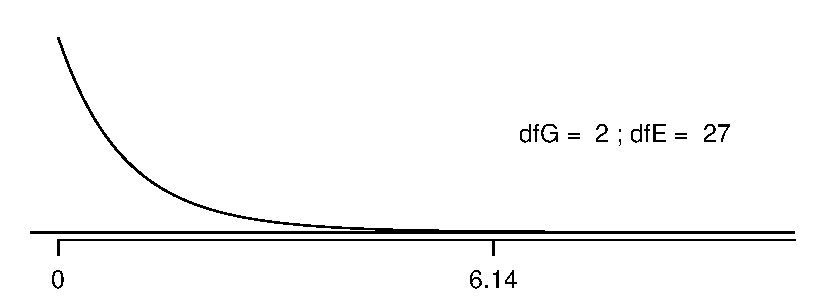
\includegraphics[width=0.9\textwidth]{5-5_anova/figures/aldrin/f}

\end{frame}

%%%%%%%%%%%%%%%%%%%%%%%%%%%%%%%%%%%

\begin{frame}
\frametitle{Conclusion - in context}

\pq{What is the conclusion of the hypothesis test?}

$\:$ \\

The data provide convincing evidence that the average aldrin concentration
\begin{enumerate}[(a)]

\item  is different for all groups.

\item on the surface is lower than the other levels.

\solnMult{is different for at least one group.}

\item is the same for all groups.

\end{enumerate}

\end{frame}

%%%%%%%%%%%%%%%%%%%%%%%%%%%%%%%%%%%

\begin{frame}
\frametitle{Conclusion}

\begin{itemize}

\item  If p-value is small (less than $\alpha$), reject $H_0$. The data provide convincing evidence that at least one mean is different from (but we can't tell which one).

\pause

\item If p-value is large, fail to reject $H_0$. The data do not provide convincing evidence that at least one pair of means are different from each other, the observed differences in sample means are attributable to sampling variability (or chance).

\end{itemize}

\end{frame}

%%%%%%%%%%%%%%%%%%%%%%%%%%%%%%%%%%%

\subsection{Checking conditions}

%%%%%%%%%%%%%%%%%%%%%%%%%%%%%%%%%%%

\begin{frame}[fragile]
\frametitle{(1) independence}

\dq{Does this condition appear to be satisfied?}

\soln{\only<2>{In this study the we have no reason to believe that the aldrin concentration won't be independent of each other.}}

\end{frame}

%%%%%%%%%%%%%%%%%%%%%%%%%%%%%%%%%%%

\begin{frame}[fragile]
\frametitle{(2) approximately normal}

\dq{Does this condition appear to be satisfied?}

\begin{center}
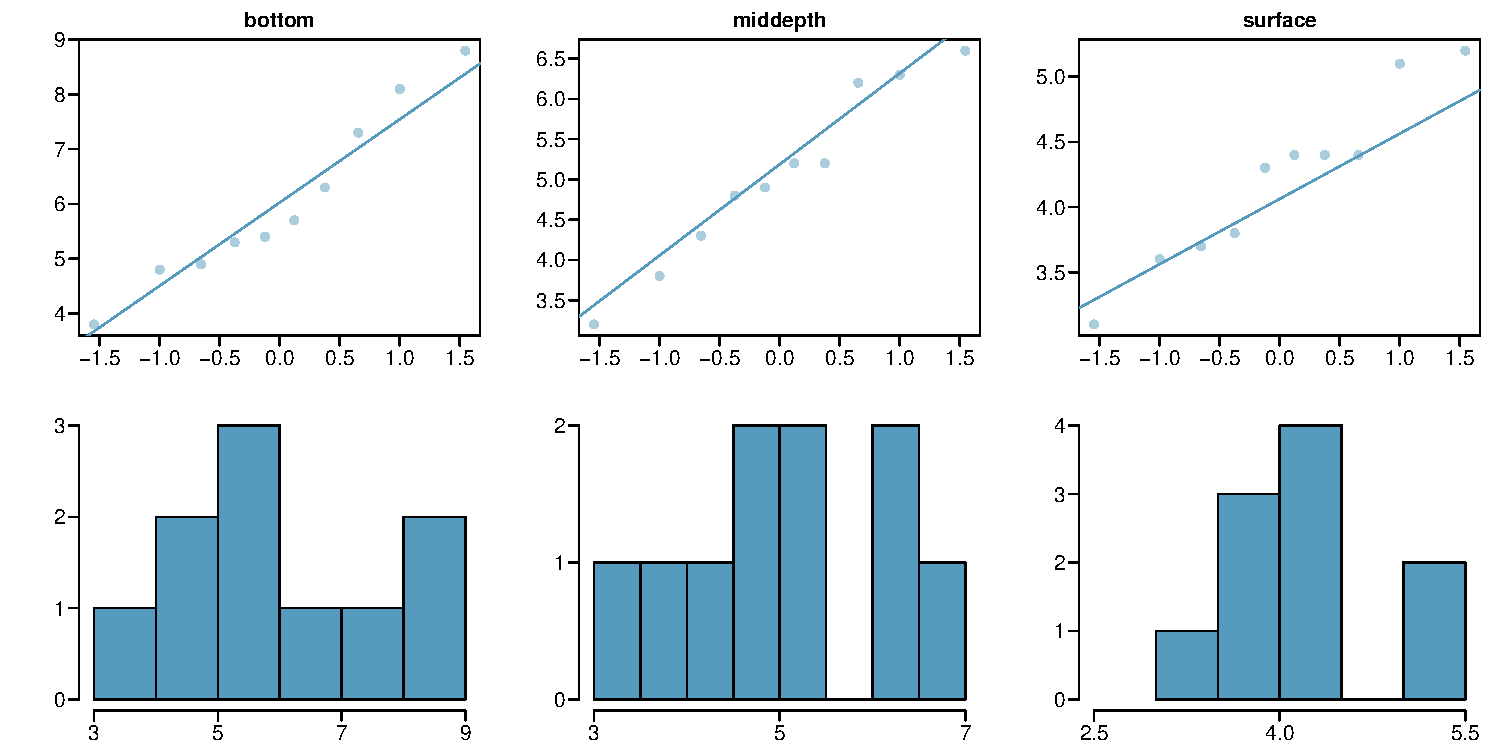
\includegraphics[width=\textwidth]{5-5_anova/figures/aldrin/normal}
\end{center}

\end{frame}

%%%%%%%%%%%%%%%%%%%%%%%%%%%%%%%%%%%

\begin{frame}[fragile]
\frametitle{(3) constant variance}

\dq{Does this condition appear to be satisfied?}

\begin{center}
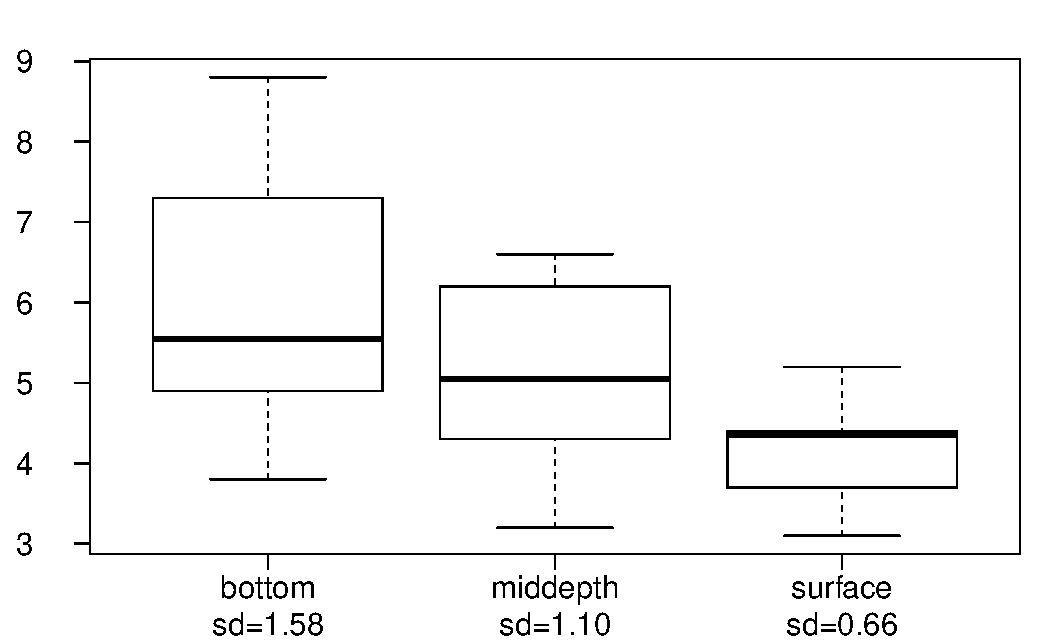
\includegraphics[width=0.7\textwidth]{5-5_anova/figures/aldrin/homo}
\end{center}

\end{frame}

%%%%%%%%%%%%%%%%%%%%%%%%%%%%%%%%%%%

\subsection{Multiple comparisons \& Type 1 error rate}

%%%%%%%%%%%%%%%%%%%%%%%%%%%%%%%%%%%

\begin{frame}
\frametitle{Which means differ?}

\begin{itemize}

\item Earlier we concluded that at least one pair of means differ. The natural question that follows is ``which ones?"

\pause

\item We can do two sample $t$ tests for differences in each possible pair of groups.

\pause

\end{itemize}

\dq{Can you see any pitfalls with this approach?}

\pause

\begin{itemize}

\item When we run too many tests, the Type 1 Error rate increases.

\item This issue is resolved by using a modified significance level.

\end{itemize}

\end{frame}

%%%%%%%%%%%%%%%%%%%%%%%%%%%%%%%%%%%

\begin{frame}
\frametitle{Multiple comparisons}

\begin{itemize}

\item The scenario of testing many pairs of groups is called \hl{multiple comparisons}.

\pause

\item The \hl{Bonferroni correction} suggests that a more \red{stringent} significance level is more appropriate for these tests:

\[ \alpha^\star = \alpha / K \]

where $K$ is the number of comparisons being considered.

\pause

\item If there are $k$ groups, then usually all possible pairs are compared and $K = \frac{k (k - 1)}{2}$.

\end{itemize}

\end{frame}

%%%%%%%%%%%%%%%%%%%%%%%%%%%%%%%%%%%

\begin{frame}
\frametitle{Determining the modified $\alpha$}

\pq{In the aldrin data set depth has 3 levels: bottom, mid-depth, and surface. If $\alpha = 0.05$, what should be the modified significance level for two sample $t$ tests for determining which pairs of groups have significantly different means?}

\begin{enumerate}[(a)]
\item $\alpha^* = 0.05$
\item $\alpha^* = 0.05 / 2 = 0.025$
\solnMult{$\alpha^* = 0.05 / 3 = 0.0167$}
\item $\alpha^* = 0.05 / 6 = 0.0083$
\end{enumerate}

\end{frame}

%%%%%%%%%%%%%%%%%%%%%%%%%%%%%%%%%%%

\begin{frame}
\frametitle{Which means differ?}

\pq{Based on the box plots below, which means would you expect to be significantly different?}

\twocol{0.6}{0.4}{
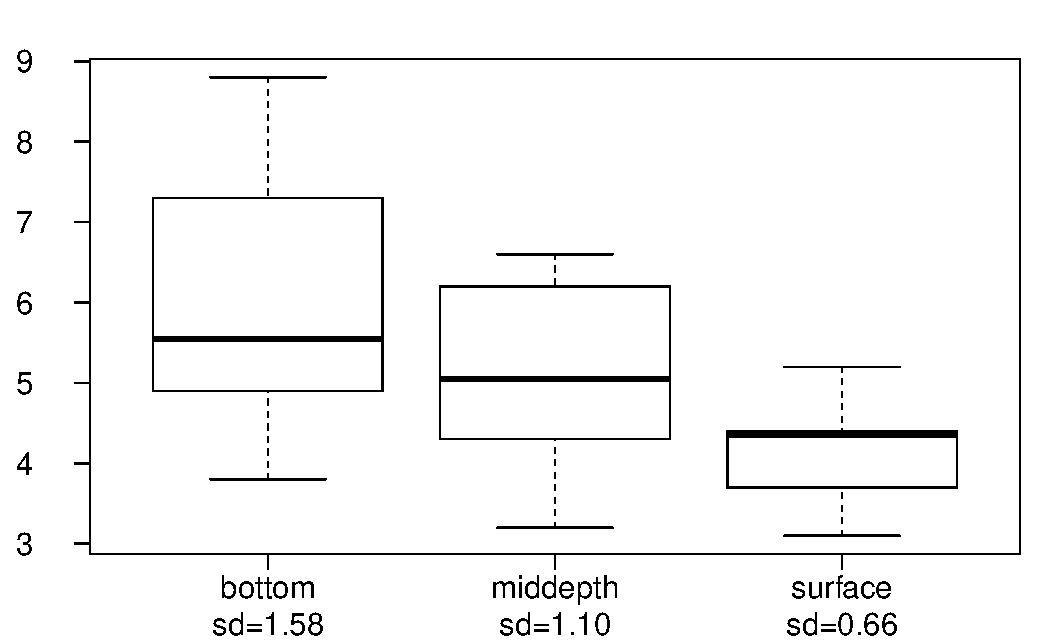
\includegraphics[width=\textwidth]{5-5_anova/figures/aldrin/homo}
}
{
\begin{enumerate}[(a)]
\item bottom \& surface
\item bottom \& mid-depth
\item mid-depth \& surface
\item bottom \& mid-depth; mid-depth \& surface
\item bottom \& mid-depth; bottom \& surface; mid-depth \& surface
\end{enumerate}
}

\end{frame}

%%%%%%%%%%%%%%%%%%%%%%%%%%%%%%%%%%

\begin{frame}
\frametitle{Which means differ? (cont.)}

If the ANOVA assumption of equal variability across groups is satisfied, we can use the data from all groups to estimate variability:
 
\begin{itemize}

\item Estimate any within-group standard deviation with $\sqrt{MSE}$, which is $s_{pooled}$

\item Use the error degrees of freedom, $n - k$, for $t$-distributions

\end{itemize}

\formula{Difference in two means: after ANOVA}{
\[ SE = \sqrt{  \frac{\sigma_1^2}{n_1} + \frac{\sigma_2^2}{n_2} } \approx \sqrt{ \frac{MSE}{n_1} + \frac{MSE}{n_2} } \]
}

\end{frame}

%%%%%%%%%%%%%%%%%%%%%%%%%%%%%%%%%%

\begin{frame}
\frametitle{}

\dq{Is there a difference between the  average aldrin concentration at the bottom and at mid depth?}

\twocol{0.4}{0.7}{
{\scriptsize
\begin{center}
\begin{tabular}{l | c c c}
		& n	& mean	& sd		\\
\hline
bottom	& 10	& \red{6.04}	& 1.58 \\
middepth& 10	& \red{5.05}	& 1.10 \\
surface	& 10	& 4.2 	& 0.66 \\
\hline
overall	& 30	& 5.1		& 1.37
\end{tabular}
\end{center}
}
}
{
{\scriptsize
\begin{center}
\begin{tabular}{l rrrrr}
\hline
 			& Df 	& Sum Sq	& Mean Sq 	& F value 	& Pr($>$F) \\ 
\hline
depth 		& 2 	& 16.96 	& 8.48 		& 6.13 	& 0.0063 \\ 
Residuals 	& \red{27} 	& 37.33 	& \red{1.38} 		&  		&  \\ 
\hline
Total			& 29	& 54.29 \\
\end{tabular}
\end{center}
}
}

\begin{eqnarray*}
T_{df_E} &=& \frac{(\bar{x}_{bottom} - \bar{x}_{middepth})}{\sqrt{ \frac{MSE}{n_{bottom}} + \frac{MSE}{n_{middepth}} }} \\ 
\pause
T_{27} &=& \frac{( 6.04 - 5.05 )}{\sqrt{ \frac{1.38}{10} + \frac{1.38}{10} }} = \frac{0.99}{0.53}  =1.87 \\
\pause
0.05 &<& p-value < 0.10 \qquad \text{{\footnotesize (two-sided)}} \\
\pause
\alpha^\star &=& 0.05 / 3 = 0.0167
\end{eqnarray*}

\pause
{\small Fail to reject $H_0$, the data do not provide convincing evidence of a difference between the average aldrin concentrations at bottom and mid depth.}

\end{frame}

%%%%%%%%%%%%%%%%%%%%%%%%%%%%%%%%%%

\begin{frame}
\frametitle{}

\app{Pairwise comparisons}{Is there a difference between the  average aldrin concentration at the bottom and at surface?}

\pause

\soln{
\begin{eqnarray*}
T_{df_E} &=& \frac{(\bar{x}_{bottom} - \bar{x}_{surface})}{\sqrt{ \frac{MSE}{n_{bottom}} + \frac{MSE}{n_{surface}} }} \\ 
\pause
T_{27} &=& \frac{( 6.04 - 4.02 )}{\sqrt{ \frac{1.38}{10} + \frac{1.38}{10} }} = \frac{2.02}{0.53}  =3.81 \\
\pause
p-value &<& 0.01 \qquad \text{{\footnotesize (two-sided)}} \\
\pause
\alpha^\star &=& 0.05 / 3 = 0.0167
\end{eqnarray*}
\pause
{\small Reject $H_0$, the data provide convincing evidence of a difference between the average aldrin concentrations at bottom and surface.}
}

\end{frame}

%%%%%%%%%%%%%%%%%%%%%%%%%%%%%%%%%%


%%%%%%%%%%%%%%%%%%%%%%%%%%%%%%%%%%%%
% End document
%%%%%%%%%%%%%%%%%%%%%%%%%%%%%%%%%%%%

\end{document}